\documentclass[preprint,authoryear,number]{elsarticle}
\usepackage{setspace}
\setlength{\parskip}{0.5em}
\setlength{\footnotesep}{12pt}

\usepackage[utf8]{inputenc}
\usepackage[T1]{fontenc}
\usepackage{amsmath,amssymb}
\usepackage{graphicx}
\usepackage{booktabs}
\usepackage{multirow}
\usepackage{xcolor}
\usepackage{hyperref}
\usepackage{siunitx}
\usepackage{lineno}
\usepackage{natbib}

\modulolinenumbers[5]
\linenumbers

\journal{ISPRS Journal of Photogrammetry and Remote Sensing}

\begin{document}

\begin{frontmatter}

\title{Stratified machine-learning bias correction of FABDEM transfers between contrasting Chilean climate regimes: evidence from ICESat-2 over Mediterranean and humid temperate watersheds}

\author[usach]{Francisco Parra~O.\corref{cor1}}
\ead{francisco.parra.o@usach.cl}
\cortext[cor1]{Corresponding author}

\address[usach]{Universidad de Santiago de Chile (USACH), Santiago, Chile}

\begin{abstract}
Global 30-m DEMs such as FABDEM achieve aggregate RMSE near \SI{2.5}{\meter}, but it is unclear whether this hides regionally learnable bias and whether a correction transfers across climate regimes. We use 135{,}350 ICESat-2 ATL08 v7 footprints over central-south Chile (34--39$^{\circ}$S) as LiDAR ground truth, training XGBoost on $h_{te} - \mathrm{fabdem}$ with 33 geomorphometric, hydrological and satellite features under spatial-block cross-validation (\SI{10}{\kilo\meter} blocks, $K=5$). The correction reduces Mediterranean RMSE from 3.054 to \SI{2.483}{\meter} ($-18.7\%$) and eliminates a $+\SI{1.0}{\meter}$ bias; stratified gains reach $-41.6\%$ in dense vegetation and $-33.8\%$ above \SI{3000}{\meter}. A Hawker-style RandomForest re-trained on the same data reaches \SI{2.510}{\meter} ($-17.8\%$), within \SI{1.1}{\percent} of XGBoost---indicating that the principal source of the gain is regional re-training on local ATL08 ground truth, not the choice of learner. Eight-regime OOD evaluation shows conditional transfer along two pre-conditions (Andean-style relief plus positive FABDEM canopy bias): favourable on humid temperate Chile ($-22.2\%$) and a four-site tropical montane Andean panel from Colombia to Bolivia (aggregate $-14.7\%$, $n{=}5{,}308$); degradation on Vietnam Mekong Delta ($+5.8\%$, lacks Andean relief) and Atacama ($+54\%$ on already-accurate \SI{0.6}{\meter} FABDEM, lacks canopy bias). The corrected DEM (Cloud-Optimized GeoTIFF, CC BY-NC-4.0), training dataset, trained model and pipeline code are released as open artefacts.
\end{abstract}

\begin{keyword}
FABDEM \sep bias correction \sep ICESat-2 ATL08 \sep XGBoost \sep spatial-block cross-validation \sep Chile \sep out-of-distribution generalisation
\end{keyword}

\end{frontmatter}

%% Highlights (submitted as separate file)
%% - Regional XGBoost correction cuts FABDEM RMSE from 3.05 m to 2.48 m on 77,501 ATL08 footprints under spatial-block CV
%% - Stratified gains: -41.6% in dense vegetation, -33.8% above 3000 m, -19.1% in floodplains
%% - Cross-regime transferability is bounded across eight climate regimes: humid temperate Chile -22.2%, four-site tropical montane Andean panel (Co/Ec/Pe/Bo) -14.7%; Vietnam Mekong +5.8%; Atacama +54%
%% - Regional re-training is the principal source of the gain: Hawker-style RandomForest within 1.1% of XGBoost, and FT-Transformer (SOTA tabular DL) at 2.54 m; gradient-boosted/RF dominate tabular SR-DEM at n=77k
%% - Corrected DEM has approached the ATL08 ground-truth noise floor in 12 of 16 evaluated tiles; further accuracy gains require airborne LiDAR
%% - Corrected DEM, 135k-footprint training set, model and code released openly under CC BY-NC-4.0 / MIT / CC0

%% ============================================================
\section{Introduction}
\label{sec:introduction}

Open-access global digital elevation models (DEMs) underpin essentially every contemporary application that requires terrain information at regional or continental scale, from flood inundation modelling \citep{Wing2024GlobalFlood,Hawker2024Vietnam} to land-surface processes, infrastructure planning, and earth-surface dynamics. Three decades of mission heritage---SRTM \citep{Farr2007SRTM}, ASTER GDEM, TanDEM-X \citep{Rizzoli2017TanDEMX}, ALOS World 3D, NASADEM, MERIT \citep{Yamazaki2017MERIT}, and Copernicus DEM---have progressively reduced global vertical error but have not eliminated it. Each successive product inherits, in modified form, residual biases from the underlying acquisition geometry, vegetation occlusion, and built-environment artefacts \citep{Schumann2018DEMSurvey,Hawker2018Accuracy}. The Forest And Buildings removed Copernicus DEM (FABDEM; \citealt{Hawker2022FABDEM}) is, at the time of writing, the most accurate publicly available bare-earth DEM at \SI{30}{\meter} resolution, achieving an aggregate global root mean square error (RMSE) of approximately \SI{2.5}{\meter} after a random-forest correction removes canopy and building height contributions from the Copernicus DSM. Independent benchmarks confirm FABDEM as the strongest of the freely available 30-m DEMs in flood-prone environments \citep{Meadows2024VerticalAccuracy}.

Despite this advance, two practically important questions remain only partially addressed. First, does FABDEM's aggregate $\sim$\SI{2.5}{\meter} global RMSE conceal a \emph{geographically heterogeneous} bias structure that could be exploited by targeted regional correction? Although the global random-forest model of \citet{Hawker2022FABDEM} removes the largest systematic effects, it is by design a single global function: the same correction is applied everywhere, with no regional adaptation. If FABDEM's residual error in, say, dense Andean foothill forest follows a different geomorphometric signature than its error in semi-arid Mediterranean valley terrain, then a regionally fine-tuned correction could in principle further reduce RMSE in specific terrain types. Second, can such a regional correction \emph{transfer} between climate regimes---that is, does a model trained on one terrain--vegetation regime usefully correct FABDEM in a contrasting regime \emph{without retraining}? This is a transferability question with direct implications for cost and scalability: if a Chilean-trained correction is portable, the methodology can be applied to ungauged regions where local ground truth is unavailable. Commercial alternatives such as FABDEM+ \citep{Fathom2024FABDEMPlus} exist but their methodology is proprietary, precluding independent evaluation of regional behaviour.

Validating either question at scale has historically been bottlenecked by access to high-precision ground-truth elevation. Airborne LiDAR is the gold standard but is expensive, geographically uneven, and frequently unavailable for the specific basins of interest. ICESat-2, launched in 2018, has begun to change this landscape. The ATLAS instrument acquires along-track photon-counting altimetry at cm-level vertical precision over a global, repeat-orbit footprint \citep{Markus2017ICESat2}, with calibration and geolocation accuracy independently validated against in situ measurements over flat ice surfaces \citep{Brunt2021ICESat2Accuracy,Magruder2021ICESat2Performance}. The ATL08 land-and-vegetation product \citep{Neuenschwander2019ATL08} provides quality-controlled ground-classified segments at $\sim$\SI{100}{\meter} along-track resolution with \SI{17}{\meter} circular footprint. ATL08 thus offers a satellite-borne, cm-precision LiDAR-equivalent ground truth that scales globally and refreshes every $\sim$91 days. The relevant cost is no longer access---it is engineering: extracting, quality-filtering, datum-correcting (ATL08 reports ellipsoidal heights; FABDEM uses orthometric EGM2008 heights), and feature-engineering at scale.

In this study we exploit ATL08 to construct a regional FABDEM correction and to test transferability across climate regimes. Specifically, we address three research questions:

\begin{itemize}
\item \textbf{RQ1}: Does FABDEM's bias have spatial structure that is regionally learnable from ICESat-2 ATL08 ground truth plus geomorphometric and satellite-derived features?
\item \textbf{RQ2}: How does correction performance stratify across geomorphometric (slope, curvature, HAND), climatic (NDVI, elevation), and tile-level dimensions?
\item \textbf{RQ3}: Does a regional ML correction transfer between contrasting climate regimes (Mediterranean $\leftrightarrow$ humid temperate) \emph{without retraining}?
\end{itemize}

We assemble 135{,}350 ICESat-2 ATL08 v7 ground-classified footprints over ten $1^{\circ} \times 1^{\circ}$ FABDEM tiles spanning central-south Chile (34--39$^{\circ}$S), engineer 33 features per footprint (geomorphometric, hydrological, and Sentinel-1/2 derived), and train XGBoost regression \citep{Chen2016XGBoost} on the residual $h_{te} - \mathrm{fabdem}$ (after EGM2008 datum correction; \citealt{Pavlis2012EGM2008}) with Optuna hyperparameter optimisation \citep{Akiba2019Optuna} under spatial-block cross-validation \citep{Roberts2017SpatialCV} to suppress autocorrelation leakage. We then apply the Mediterranean-trained model to humid temperate forest tiles without retraining to evaluate cross-regime transferability. Feature attribution uses SHAP values \citep{Lundberg2017SHAP} to compare what the model emphasises in each regime. We report bootstrap 95\% confidence intervals on all RMSE estimates and Diebold--Mariano tests of squared-error differentials \citep{Diebold1995ComparingPredictiveAccuracy}.

The contributions of this work are:

\begin{enumerate}
\item \textbf{An honest regional benchmark showing that regional re-training is the principal source of the RMSE gain}: we reduce spatial-block cross-validated RMSE from \SI{3.054}{\meter} to \SI{2.483}{\meter} with XGBoost---an absolute reduction of \SI{0.57}{\meter} ($-18.7\%$), block-bootstrap-honest 95\% CI on the improvement $[-20.9, -16.6]\%$, Diebold--Mariano $p < 0.001$---and eliminate a systematic $+\SI{1.0}{\meter}$ positive bias. A Hawker-style RandomForest re-trained on the same Chilean ATL08 data reaches \SI{2.510}{\meter} ($-17.8\%$), within \SI{1.1}{\percent} of XGBoost (Table~\ref{tab:dl_baseline}), establishing that the gain is attributable to regional re-training on local ground truth rather than to the choice of XGBoost over the random-forest family used by the global \citet{Hawker2022FABDEM} correction.
\item \textbf{A stratified characterisation of where the correction matters}: we show RMSE gains of $-41.6\%$ in dense vegetation, $-33.8\%$ above \SI{3000}{\meter}, and $\leq -19.1\%$ in already-accurate floodplains, with sample-sparse flat terrain extrapolating poorly.
\item \textbf{First systematic empirical characterisation, to our knowledge, of cross-regime transferability of an ML FABDEM correction, including its operational boundaries}: the Mediterranean-trained model achieves a further $-22.2\%$ RMSE reduction on humid temperate Chilean forest \emph{without retraining} (Diebold--Mariano $p < 0.001$); but the same model degrades on Vietnam Mekong Delta ($+5.8\%$) and Atacama ($+54\%$ on an already-accurate FABDEM at \SI{0.6}{\meter}). SHAP attribution shifts from drainage features to 3D shape descriptors in the favourable transfer, consistent with the model exploiting physically grounded terrain--error relationships when both Andean-style relief and a positive FABDEM canopy bias are present in the target regime.
\item \textbf{An open artefact release}---corrected COG, training dataset, trained model, and pipeline code (under CC BY-NC-4.0 inherited from FABDEM)---that positions ICESat-2 ATL08 as scalable LiDAR-equivalent ground truth for regional DEM refinement elsewhere.
\end{enumerate}

The remainder of the paper is organised as follows. Section~\ref{sec:study_area} describes the study area, including the contrasting climate regimes and the June 2023 atmospheric-river event that motivated the choice of basins. Section~\ref{sec:data} details the data sources. Section~\ref{sec:methods} specifies the methodology and pipeline. Section~\ref{sec:results} presents results, including stratified analysis and the out-of-distribution transferability test. Section~\ref{sec:discussion} discusses where the correction matters and what the SHAP-attribution shifts imply about physical interpretability and scope of transferability. Section~\ref{sec:conclusions} concludes and Section~\ref{sec:data_availability} lists data and code availability.


%% ============================================================
\section{Study area}
\label{sec:study_area}

The study area covers $\sim$700{,}000\,km$^{2}$ of central-south Chile between 34$^{\circ}$S and 39$^{\circ}$S (Fig.~\ref{fig:study_area}). At these latitudes the country is a narrow $\sim$\SI{220}{\kilo\meter} strip from Pacific coast to the Andean drainage divide, and the steep west--east climatic and topographic gradient creates a natural laboratory for terrain-correction studies: lowland coastal plain, agricultural Central Valley, pre-Andean foothills, and high Andes above \SI{3000}{\meter} all occur within each $1^{\circ}$ latitude band. We sample this transect with ten contiguous $1^{\circ} \times 1^{\circ}$ FABDEM tiles (S35W071 to S39W073), grouped into two contrasting climate regimes for the experimental design.

The \textbf{Mediterranean regime} comprises six tiles (S35W071, S35W072, S36W071, S36W072, S37W071, S37W072) spanning the Mataquito and Maule river basins (34--37$^{\circ}$S). Climate is Mediterranean \emph{sensu stricto}---dry summers, wet winters concentrated in May--August---with mean annual precipitation increasing from $\sim$\SI{400}{\milli\meter} in the north to $\sim$\SI{900}{\milli\meter} at the southern boundary. Land cover is a mosaic of intensive agriculture (vineyards, fruit orchards, cereals) in the Central Valley, sclerophyll forest on coastal-range and pre-Andean slopes, and barren or sparsely vegetated alpine terrain above the tree line. The growing-season NDVI distribution is broad with median $\approx 0.3$, reflecting this heterogeneity, with concentrated areas of bare ground (NDVI $< 0.1$) in the upper cordillera and dense canopy (NDVI $> 0.5$) only in irrigated valleys and remnant forest patches.

The \textbf{humid temperate regime} comprises four tiles (S38W072, S38W073, S39W072, S39W073) spanning the B\'io-B\'io and Araucan\'ia regions (37--39$^{\circ}$S). This is the northern margin of the Valdivian temperate rainforest biome: mean annual precipitation rises to 1{,}500--3{,}000\,mm with year-round rainfall, and natural vegetation is dense evergreen-broadleaf forest dominated by \emph{Nothofagus} species. Plantation forestry (\emph{Pinus radiata}, \emph{Eucalyptus}) covers a substantial fraction of the coastal range and central valley. Growing-season NDVI distribution is shifted upward, median $\approx 0.6$, with very dense canopy (NDVI $> 0.7$) common. Topographically the regime mirrors the Mediterranean transect---coastal range, central valley, Andean foothills, high Andes---but with denser and more spatially uniform vegetation cover. The latitudinal separation of $\sim 3^{\circ}$ ($\approx \SI{330}{\kilo\meter}$) between the two regimes' centroids and the contrast in vegetation cover (NDVI $\Delta$median $\approx 0.3$) provide a clean test of cross-regime transferability.

The June 2023 atmospheric-river event over central Chile motivates the regional focus. Between 21 and 26 June 2023, an exceptionally intense frontal system---characterised by the Centro de Ciencia del Clima y la Resiliencia as the strongest of the last three decades \citep{Garreaud2024AR2023}---delivered persistent heavy precipitation over the Mediterranean regime in particular, with widespread river overflow in the Mataquito and Maule basins. CIGIDEN documented post-disaster flood extents at Licant\'en (Mataquito river mouth; \citealt{CIGIDEN2023Licanten,CIGIDEN2023MataquitoMaule}). Although the present paper focuses on DEM correction rather than flood mapping, this event provides direct policy relevance: improvement in DEM accuracy in flood-prone Chilean basins has demonstrable applications, and Section~\ref{sec:hand_check} uses the CIGIDEN Licant\'en polygons in a HAND-threshold comparison as a preliminary downstream check.

\begin{figure*}[t]
\centering

\includegraphics[width=\textwidth]{figures/F1_study_area.pdf}
\caption{Study area in central-south Chile (34--39$^{\circ}$S). The ten $1^{\circ} \times 1^{\circ}$ FABDEM tiles are grouped into Mediterranean training tiles (six tiles, Mataquito and Maule basins; orange) and humid temperate out-of-distribution tiles (four tiles, B\'io-B\'io and Araucan\'ia; blue). Inset shows the CIGIDEN Licant\'en June~2023 flood polygon at the Mataquito river mouth. Map lines delineate study tiles and do not necessarily depict accepted national boundaries.}
\label{fig:study_area}
\end{figure*}


%% ============================================================
\section{Data}
\label{sec:data}

We use five primary data sources---the bare-earth DEM under correction, the ground-truth altimetry, two satellite remote-sensing sources for feature engineering, and a geoid model for datum harmonisation---plus a derived geomorphometric feature stack computed from the DEM itself. Table~\ref{tab:data_sources} summarises the sources; the following subsections detail provenance, processing, and resulting feature count.

\subsection{FABDEM v1.2}
\label{sec:fabdem}

FABDEM v1.2 \citep{Hawker2022FABDEM} is the bare-earth DEM under correction. It is derived from Copernicus DEM GLO-30 (the upstream Digital Surface Model) by removing canopy and building height contributions with a random-forest regression trained on global LiDAR samples. Native horizontal resolution is 1\,arcsec ($\sim$\SI{30}{\meter} at our latitudes) on a geographic WGS84 (EPSG:4326) grid, and the vertical datum is orthometric EGM2008. We download the ten $1^{\circ} \times 1^{\circ}$ tiles via the Google Earth Engine asset \texttt{projects/sat-io/open-datasets/FABDEM}, yielding $\sim$137\,M pixels across the study area. The licence is CC BY-NC-4.0, which the corrected product inherits.

\subsection{ICESat-2 ATL08 v7}
\label{sec:atl08}

ICESat-2 \citep{Markus2017ICESat2} carries the ATLAS photon-counting laser altimeter (\SI{532}{\nano\meter}, \SI{10}{\kilo\hertz} pulse rate, six beams in three weak/strong pairs). The ATL08 v7 product \citep{Neuenschwander2019ATL08} aggregates ATL03 geolocated photons into $\sim$\SI{100}{\meter} along-track land segments with a \SI{17}{\meter} circular footprint and classifies returns into ground, canopy, and noise. We download all ATL08 v7 granules intersecting each tile between January 2018 and December 2025 via \texttt{earthaccess}, extract footprints inside each tile's bounding box, and apply the following quality filters (recommended by the ATL08 ATBD and consistent with prior published DEM-validation work):

\begin{itemize}
\item \texttt{terrain\_flg == 1} (segment passed terrain quality screening);
\item \texttt{n\_te\_photons} $\geq 30$ (sufficient photon support for the terrain estimate);
\item \texttt{h\_te\_uncertainty} $< \SI{10}{\meter}$ (1-$\sigma$ along-track uncertainty);
\item \texttt{segment\_snowcover == 1} and \texttt{segment\_watermask == 0} (no snow, not water);
\item \texttt{cloud\_flag\_atm} $\leq 1$ (clear-sky atmosphere).
\end{itemize}

After filtering, the retained sample is 77{,}501 footprints in the Mediterranean regime and 57{,}849 in humid temperate, for a combined dataset of 135{,}350 ground-classified footprints. The variable used as truth is \texttt{h\_te\_best\_fit} (best-fit terrain elevation), converted from WGS84 ellipsoidal to EGM2008 orthometric heights via the PROJ pipeline (EPSG:4979 $\to$ EPSG:9518) using gridded EGM2008 \citep{Pavlis2012EGM2008} with PROJ network mode enabled. The geoid undulation over the study area ranges from approximately $+18$ to $+\SI{24}{\meter}$ and applying it removes an apparent $+21$--\SI{22}{\meter} baseline offset between raw ATL08 ellipsoidal heights and FABDEM, leaving a residual mean error of approximately $+\SI{1}{\meter}$ attributable to FABDEM itself.

\subsection{Sentinel-2 L2A optical composites}
\label{sec:sentinel2}

We assemble single-season austral summer optical composites (December 2022 to February 2023) from Sentinel-2 L2A \citep{Drusch2012Sentinel2} via the Microsoft Planetary Computer STAC API. For each MGRS tile intersecting the study area we select the three least-cloudy granules with cloud cover below 20\%, stack them with \texttt{stackstac} at \SI{60}{\meter} resolution on the UTM 19S projection (EPSG:32719), and compute the per-pixel median across the time stack for bands B02 (blue), B03 (green), B04 (red), B08 (NIR), B11 (SWIR-1), and B12 (SWIR-2). From these we derive five spectral indices: NDVI (vegetation), NDWI (water/wetness), NDMI (moisture), BSI (bare-soil), and NDBI (built-up/non-vegetation). The \SI{60}{\meter} output resolution is a deliberate trade-off: lowering Sentinel-2 from native 10--\SI{20}{\meter} to \SI{60}{\meter} reduces memory footprint by an order of magnitude for the per-tile compute, with minimal information loss for point-sampling at ICESat-2 footprint locations (which are themselves spatial integrations over a \SI{17}{\meter} footprint).

\subsection{Sentinel-1 RTC SAR composites}
\label{sec:sentinel1}

We assemble parallel C-band SAR backscatter composites from Sentinel-1 RTC products \citep{Torres2012Sentinel1} via Planetary Computer. For each tile we retain up to 12 dual-polarisation (VV $+$ VH) granules from the same December 2022--February 2023 window, compute the per-pixel median, convert to decibels ($\sigma^{0}$ in dB), and derive the VV/VH ratio. Final outputs at \SI{60}{\meter} UTM 19S are three rasters: \texttt{s1\_vv\_db}, \texttt{s1\_vh\_db}, and \texttt{s1\_vv\_vh\_ratio}. SAR backscatter complements the optical composite by being weather-independent and sensitive to surface roughness and dielectric properties (vegetation moisture content), which are partially decoupled from optical vegetation greenness.

\subsection{Geomorphometric and hydrological features (SurtGis)}
\label{sec:surtgis}

From each tile's FABDEM raster we derive a stack of geomorphometric and hydrological terrain features using SurtGis \citep{SurtGis2026}, an open-source Rust geospatial library that exposes streaming, parallel implementations of standard algorithms. The two batch operations \texttt{surtgis terrain all} and \texttt{surtgis hydrology all} produce, in a single pass per tile:

\begin{itemize}
\item \textbf{Slope, aspect (sin/cos), hillshade}---standard first-derivative quantities;
\item \textbf{Curvature (general, profile, planform), TPI, TRI, VRM, dev, convergence}---second-derivative and ruggedness descriptors;
\item \textbf{Openness positive/negative, sky-view factor (SVF)}---3D form descriptors capturing local concavity/convexity at longer length scales \citep{Yokoyama2002Openness};
\item \textbf{MRVBF, MRRTF}---Multi-Resolution Valley Bottom / Ridge Top Flatness \citep{Gallant2003MRVBF};
\item \textbf{Geomorphons}---10-class landform classification \citep{Jasiewicz2013Geomorphons};
\item \textbf{HAND}---Height Above Nearest Drainage \citep{Nobre2011HAND}, a drainage-relative elevation quantity widely used in flood-prone areas;
\item \textbf{TWI}---Topographic Wetness Index \citep{Beven1979TOPMODEL};
\item \textbf{Flow direction (D8 and D-infinity), flow accumulation (single and multi-flow), filled DEM, stream network}---standard hydrological derivatives;
\item \textbf{Valley depth}---distance from each pixel to the nearest ridge top elevation.
\end{itemize}

In total, after de-duplication, this yields 25 geomorphometric and hydrological rasters per tile in the FABDEM native EPSG:4326 / \SI{30}{\meter} grid. Each is sampled at footprint locations during the feature-stack assembly step.

\subsection{Final feature stack}
\label{sec:feature_stack}

Combining the satellite-derived (5 Sentinel-2 indices $+$ 3 Sentinel-1 SAR statistics) and DEM-derived (25 SurtGis outputs) features yields a \textbf{33-feature stack} per footprint after sampling. The regression target is the EGM2008-corrected residual
\begin{equation}
y = h_{\text{te,orthometric}} - h_{\text{fabdem}}, \quad \text{units in metres,}
\label{eq:target}
\end{equation}
with values close to zero indicating an accurate FABDEM pixel and large-magnitude values signalling correctable bias. The sign convention is that positive $y$ corresponds to FABDEM underestimating the true ground surface; the empirically observed regional median is $-\SI{1}{\meter}$, consistent with the published global tendency of FABDEM to slightly \emph{overestimate} bare-earth elevation in vegetated terrain---likely a residual artefact of the upstream Copernicus DSM canopy bias incompletely removed by the global RF model. Table~\ref{tab:data_sources} lists licences and access methods for every source.

\begin{table*}[t]
\centering
\caption{Data sources used in this study. ICESat-2 ATL08 provides ground truth; FABDEM is the DEM under correction; Sentinel-1/2 and EGM2008 feed the feature stack; CIGIDEN Licant\'en is used as flood reference in the discussion.}
\label{tab:data_sources}
\footnotesize
\begin{tabular}{p{2.4cm}p{3cm}p{2cm}p{2cm}p{1.5cm}p{1.5cm}p{3cm}}
\toprule
\textbf{Source} & \textbf{Type} & \textbf{Native res.} & \textbf{Coverage} & \textbf{Format} & \textbf{License} & \textbf{Access} \\
\midrule
FABDEM v1.2 & Bare-earth DEM & 1 arcsec ($\sim$30 m) & $\pm$80$^{\circ}$ lat & GeoTIFF & CC BY-NC-4.0 & GEE \texttt{projects/sat-io/open-datasets/FABDEM} \\
ICESat-2 ATL08 v7 & Photon-derived land + canopy heights & 100~m segment, 17~m footprint & Global, 91-day repeat & HDF5 & Public domain & NASA Earthdata via \texttt{earthaccess} \\
Sentinel-2 L2A & Surface reflectance, 13 bands & 10--60 m & Global, $\sim$5-day revisit & GeoTIFF (COG) & Open (Copernicus) & Microsoft Planetary Computer STAC \\
Sentinel-1 RTC & C-band SAR backscatter $\sigma^{0}$ & 10~m & Global, $\sim$12-day revisit & GeoTIFF (COG) & Open (Copernicus) & Microsoft Planetary Computer STAC \\
EGM2008 geoid & Geoid undulation grid & 2.5$^{\prime}$ & Global & GeoTIFF & Open (NGA) & PROJ network mode (EPSG:4979$\rightarrow$9518) \\
CIGIDEN Licantén & Sentinel-derived flood polygon, jun 2023 event & Vector polygons & Licantén (35$^{\circ}$S), Mataquito mouth & Shapefile & Open (CC) & Zenodo DOI \texttt{10.5281/zenodo.13307972} \\
\bottomrule
\end{tabular}
\end{table*}



%% ============================================================
\section{Methods}
\label{sec:methods}

\subsection{Pipeline architecture}
\label{sec:pipeline}

The processing pipeline (Fig.~\ref{fig:pipeline}) is organised as a tile-parallel sequence of seven stages: (i) FABDEM tile retrieval, (ii) geomorphometric and hydrological feature derivation, (iii) Sentinel-1/2 composite assembly, (iv) ICESat-2 ATL08 granule acquisition, (v) footprint extraction and datum correction, (vi) feature-stack sampling at footprint locations, and (vii) regression target assembly. Stages (i)--(vi) execute independently per $1^{\circ}$ tile inside isolated process trees; their outputs (per-tile sample tables) are concatenated at the end. Each stage is checkpointed: if a partial output already exists with valid metadata, the stage is skipped on re-execution, which makes the pipeline robust to mid-run interruptions and incremental data additions. A \texttt{psutil}-based watchdog monitors combined RAM of the running stage plus all child processes and aborts the stage cleanly if a configurable threshold (here \SI{8}{\giga\byte}) is exceeded, preventing the long-running pipeline from competing for swap with the operating system. The watchdog never fired in production runs after the satellite-stage RAM optimisation described in Section~\ref{sec:feature_assembly} was applied.

\begin{figure*}[t]
\centering
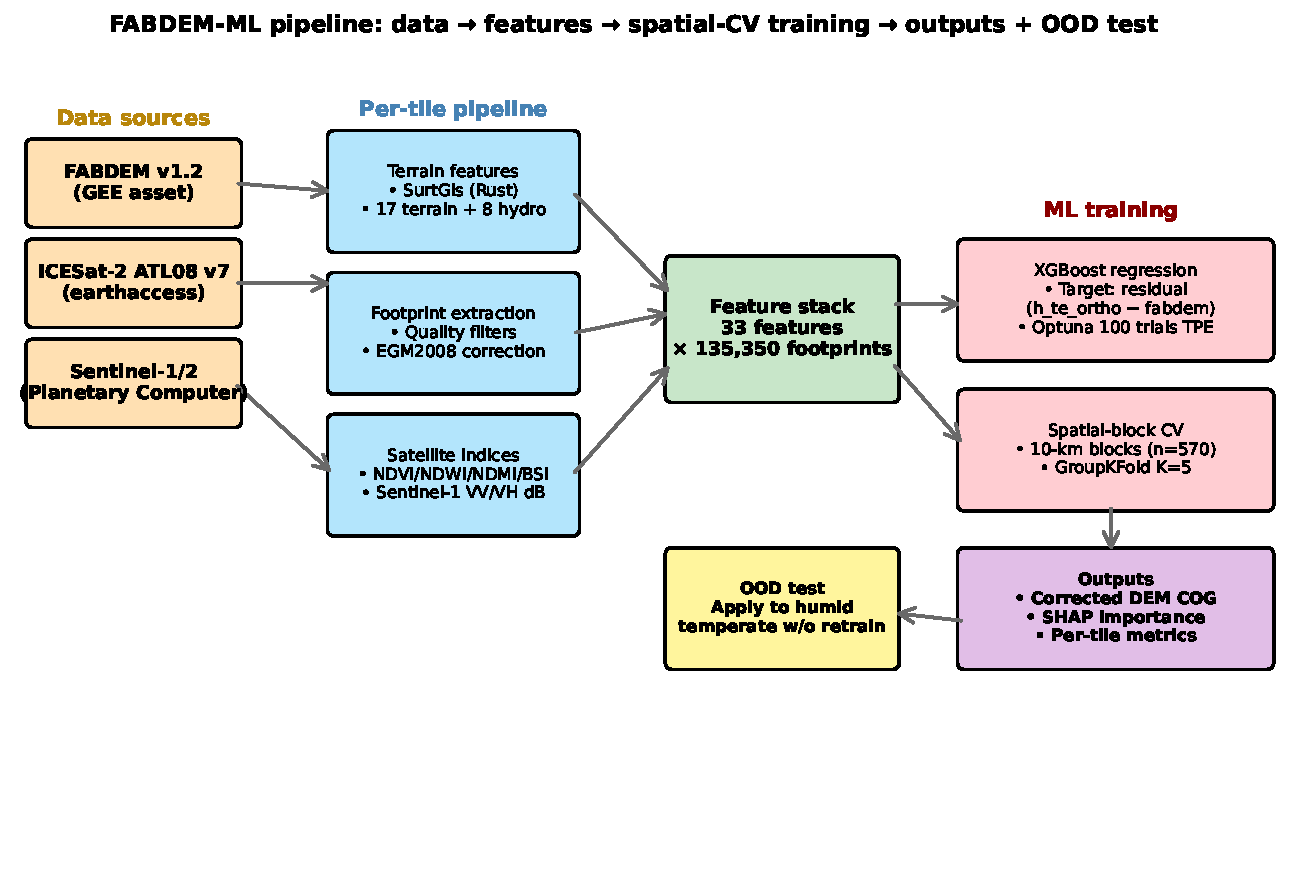
\includegraphics[width=\textwidth]{figures/F2_pipeline_flowchart.pdf}
\caption{End-to-end processing pipeline. Stages (i)--(vi) execute independently per $1^{\circ}$ FABDEM tile; per-tile sample tables are concatenated for training. Each stage is checkpointed (skipped on resume if output exists) and supervised by a \texttt{psutil}-based RAM watchdog. ATL08 footprints are converted from WGS84 ellipsoidal to EGM2008 orthometric heights via PROJ network mode before the regression target is assembled.}
\label{fig:pipeline}
\end{figure*}

\subsection{Footprint extraction and EGM2008 datum correction}
\label{sec:egm2008}

For each tile we download every ATL08 v7 granule whose bounding polygon intersects the tile geometry, then iterate through the six ATLAS beams (\texttt{gt1l}--\texttt{gt3r}). For each land-segment record we retain the longitude, latitude, best-fit terrain height (\texttt{terrain/h\_te\_best\_fit}), per-segment uncertainty (\texttt{terrain/h\_te\_uncertainty}), and the quality flags listed in Section~\ref{sec:atl08}. Quality filtering retains records satisfying simultaneously: \texttt{terrain\_flg} $= 1$, \texttt{n\_te\_photons} $\geq 30$, \texttt{h\_te\_uncertainty} $< \SI{10}{\meter}$, \texttt{segment\_snowcover} $= 1$, \texttt{segment\_watermask} $= 0$, \texttt{cloud\_flag\_atm} $\leq 1$. These thresholds follow \citet{Neuenschwander2019ATL08} for surface terrain analysis and screen out water bodies, snow-covered surfaces, cloud-contaminated retrievals, and low-photon-count segments where the best-fit elevation is poorly constrained.

ATL08 reports heights above the WGS84 ellipsoid, whereas FABDEM uses orthometric heights referenced to the EGM2008 geoid \citep{Pavlis2012EGM2008}. Failing to harmonise the two leaves an apparent $\sim +\SI{22}{\meter}$ baseline offset that would entirely dominate the regression target and silently corrupt downstream analysis. We apply the conversion per footprint using the PROJ pipeline from EPSG:4979 (WGS84 3D ellipsoidal) to EPSG:9518 (WGS84 horizontal $+$ EGM2008 vertical), with PROJ network mode enabled so that the EGM2008 grid is fetched on demand. The geoid undulation varies by approximately \SI{6}{\meter} across the latitudinal extent of the study area, so the correction is per-point rather than a constant offset. The corrected heights, denoted $h_{\text{te,ortho}}$, define the regression target as the signed residual $y = h_{\text{te,ortho}} - h_{\text{fabdem}}$ in metres.

\subsection{Feature-stack assembly with CRS-aware sampling}
\label{sec:feature_assembly}

FABDEM and its derived terrain features (Section~\ref{sec:surtgis}) reside on a geographic grid (EPSG:4326, $\sim$\SI{30}{\meter}), while the Sentinel-1/2 composites (Sections~\ref{sec:sentinel2}--\ref{sec:sentinel1}) reside on a projected grid (EPSG:32719 UTM 19S, \SI{60}{\meter}). For each footprint we reproject the (lon, lat) coordinate pair into each source raster's native CRS and sample the underlying pixel value with nearest-neighbour interpolation via \texttt{rasterio}. This avoids unnecessary raster reprojection at the per-pixel scale, which would propagate resampling artefacts into the feature values. One feature, \texttt{stream\_network}, is a sparse binary indicator produced by the SurtGis hydrology stream-extraction; for non-stream cells the SurtGis output is NaN, which is semantically equivalent to ``no stream present'' and is therefore reassigned to zero before regression to retain its informational value as a present/absent indicator.

\subsection{XGBoost regression with Optuna hyperparameter tuning}
\label{sec:xgboost}

We train gradient-boosted decision trees with XGBoost \citep{Chen2016XGBoost} on the 33-feature stack to predict the residual target $y$. Hyperparameters are tuned by Optuna \citep{Akiba2019Optuna} using a Tree-structured Parzen Estimator (TPE) sampler over 100 trials, with the objective function defined as the mean spatial-cross-validated out-of-fold RMSE (Section~\ref{sec:spatial_cv}). The search space covers \texttt{max\_depth} $\in [3, 9]$, \texttt{learning\_rate} $\in [0.005, 0.2]$ (log scale), \texttt{subsample} $\in [0.5, 1.0]$, \texttt{colsample\_bytree} $\in [0.5, 1.0]$, \texttt{min\_child\_weight} $\in [1, 20]$, \texttt{reg\_lambda} $\in [10^{-3}, 10^{2}]$ (log scale), \texttt{reg\_alpha} $\in [10^{-4}, 10]$ (log scale), and \texttt{gamma} $\in [0, 5]$. The number of boosting rounds is capped at 1{,}000 with early stopping after 30 rounds without validation-RMSE improvement. The final selected hyperparameters (Table~\ref{tab:hyperparams}) describe deep trees (\texttt{max\_depth} $= 9$) coupled with aggressive regularisation (\texttt{min\_child\_weight} $= 14$, \texttt{reg\_lambda} $\approx 7.4$, \texttt{gamma} $\approx 2.2$) and a low learning rate ($\approx 0.011$), a combination consistent with a smooth target manifold that benefits from depth but is prone to overfit under standard regularisation choices.

\input{tables/T2_hyperparameters}

The regression operates on raw, untransformed features. XGBoost handles missing values internally by routing them along the default branch learned during split selection, which is convenient because Sentinel-1/2 composite pixels can be NaN where all input scenes are cloud-flagged. We rely on this behaviour rather than imputing values that would inject false information.

\subsection{Spatial-block cross-validation}
\label{sec:spatial_cv}

Per-pixel cross-validation with random folds is inappropriate here because ICESat-2 ATL08 footprints exhibit strong along-track spatial autocorrelation: adjacent \SI{100}{\meter} segments share atmospheric conditions, drainage context, and reference orbit, making nearby footprints near-duplicates from the model's perspective. Random partitions would assign these clusters to both train and test sets and yield optimistic generalisation estimates \citep{Roberts2017SpatialCV}. We therefore use \textbf{spatial-block cross-validation}: footprints are projected to UTM 19S, integer-divided by \SI{10000}{\meter} to assign a $\SI{10}{\kilo\meter} \times \SI{10}{\kilo\meter}$ block index, and these block indices are used as group labels in scikit-learn's \texttt{GroupKFold} partitioning with $K = 5$ folds. The procedure ensures that all footprints within a \SI{10}{\kilo\meter} tile are kept in the same fold, so that the model is always evaluated on geographically distinct ground from where it was trained. Across the Mediterranean dataset, 570 unique blocks are created from the 77{,}501 footprints, giving approximately 114 blocks per fold (with some imbalance from variable block density). To quantify the magnitude of autocorrelation leakage we also report random $K$-fold CV (which loses the spatial constraint) for direct comparison; the gap is small (3.5\% RMSE inflation under random CV), indicating that \SI{10}{\kilo\meter} blocks are large enough to suppress local-track contamination without being so large that they remove genuine model capacity. A \SI{5}{\kilo\meter} vs \SI{10}{\kilo\meter} vs \SI{20}{\kilo\meter} sensitivity test reported in Section~\ref{sec:sensitivity_baselines} yields RMSE differences below \SI{0.05}{\meter} across the full range, supporting the \SI{10}{\kilo\meter} choice as primary reporting block size.

\subsection{Tabular deep-learning baselines}
\label{sec:dl_baselines}

To verify empirically that XGBoost is a competitive learner on this tabular regression problem rather than a default selection, we train two deep-learning baselines on identical spatial-CV folds. The first is a three-layer multilayer perceptron with 256, 256 and 128 hidden units, ReLU activations, dropout 0.2 between layers, optimised with AdamW (learning rate $10^{-3}$, weight decay $10^{-4}$, batch size 2048) under MSE loss; training is capped at 200 epochs with early stopping on a 20\% random validation split of each training fold (patience 20 epochs). The second is TabNet \citep{Arik2021TabNet}, a transformer-style attentive tabular learner, with $n_d = n_a = 32$ feature dimensions, four sequential decision steps, $\gamma = 1.3$, and Adam at learning rate $2 \times 10^{-2}$ with batch size 4096. Both models receive feature-wise standardised inputs fit on each training fold and ingest the same 33-feature stack as XGBoost; missing values are median-imputed per column. Random seeds are fixed at 42 for all stochastic operations. The comparison appears in Section~\ref{sec:sensitivity_baselines}.

\subsection{Feature attribution via SHAP}
\label{sec:shap}

Per-feature importance is computed using the SHAP TreeExplainer \citep{Lundberg2017SHAP}, which exploits the tree structure to compute exact Shapley values in polynomial time. To keep memory and computation tractable on the full 77{,}501-row Mediterranean training set we draw a uniform random sample of 8{,}000 footprints (seed 42) and compute SHAP values for the final, hyperparameter-tuned model trained on the complete training set. Reported feature importance is the mean absolute SHAP value across that sample, which preserves both the magnitude and the rank of feature contributions while remaining computationally inexpensive. The same procedure is repeated on a separate 8{,}000-row sample drawn from the humid temperate dataset to enable the cross-regime comparison reported in Section~\ref{sec:results}.

\subsection{Out-of-distribution evaluation}
\label{sec:ood_method}

To test whether the regional model generalises beyond its training regime, we apply the Mediterranean-trained XGBoost model directly to the humid temperate dataset without any retraining or fine-tuning. Specifically, we load the booster fit on the complete 77{,}501-footprint Mediterranean training set (the same model used for inference and SHAP attribution) and predict residuals for the 57{,}849 humid temperate footprints. The corrected elevation is computed as $h_{\text{corrected}} = h_{\text{fabdem}} + \hat{y}$ and compared against the ATL08 ground truth via RMSE, MAE, signed bias, and per-pixel sign comparison. This is a true out-of-distribution test in the strict statistical sense: no humid temperate footprint or feature ever enters the training pipeline. Statistical significance of the squared-error reduction is assessed with a Diebold--Mariano test on the per-footprint squared-error differential, and per-pixel improvement frequency is tested with a one-sided binomial test against the null hypothesis of equal correction/degradation rates.

\subsection{Raster-wide inference}
\label{sec:raster_inference}

To produce the distributable corrected DEM (Section~\ref{sec:data_availability}) we apply the trained model to every pixel of the FABDEM raster across the six Mediterranean tiles. Each feature raster is opened lazily; for those already on the FABDEM grid (terrain and hydrology layers) values are read directly, while satellite layers in EPSG:32719 are reprojected on the fly to the FABDEM grid using bilinear resampling with \texttt{rasterio.warp.reproject}. A per-tile dense feature stack is assembled in float32, fed to the XGBoost booster via \texttt{xgb.DMatrix} with explicit \texttt{missing = NaN}, and the predicted residual is added to the corresponding FABDEM pixel to produce the corrected elevation. Output is written as a tiled Cloud-Optimized GeoTIFF with \texttt{deflate} compression, predictor 2, internal block size $512 \times 512$, and average-resampled overviews at decimation levels $[2, 4, 8, 16, 32]$. The six per-tile COGs are mosaicked into a single $7{,}422 \times 11{,}133$ raster (\texttt{mm\_corrected.tif}, \SI{282}{\mega\byte}) using SurtGis \texttt{mosaic}, which preserves the COG structure of the inputs.

\subsection{Software, versions, and reproducibility}
\label{sec:software}

The Python environment used throughout is: Python 3.12, XGBoost 3.1.1, Optuna 4.6.0, scikit-learn 1.8.0, SHAP 0.50.0, rasterio 1.4.x, pyproj 3.6.x (PROJ network mode enabled for the EGM2008 grid), \texttt{earthaccess} 0.18.0 for ATL08, \texttt{pystac-client} and \texttt{stackstac} for Planetary Computer access. Terrain and hydrology features are computed with SurtGis 0.7.0 \citep{SurtGis2026}, an open-source Rust library that exposes streaming, parallel implementations of standard geomorphometric algorithms with bounded memory per tile. A fixed random seed (42) is used for the Optuna sampler, all train/test partitions, the SHAP subsampling, and the 2{,}000-resample bootstrap that produces the confidence intervals reported in Section~\ref{sec:results}. The complete pipeline, including the tile orchestrator with checkpointing and watchdog, is released under an open licence at the repository given in Section~\ref{sec:data_availability}.


%% ============================================================
\section{Results}
\label{sec:results}

\subsection{Overall correction performance}
\label{sec:overall_performance}

Under spatial-block cross-validation on the Mediterranean dataset ($n = 77{,}501$ footprints, 570 unique \SI{10}{\kilo\meter} blocks, $K = 5$ folds), the XGBoost residual model reduces RMSE from \SI{3.054}{\meter} to \SI{2.483}{\meter} after correction---an absolute reduction of \SI{0.57}{\meter}, or \textbf{$-18.7\%$} in relative terms. The corresponding MAE drops from \SI{1.423}{\meter} to \SI{1.099}{\meter} ($-22.8\%$). We report two complementary forms of uncertainty on these estimates. A naive footprint-level bootstrap (2{,}000 resamples drawn from the 77{,}501 footprints) gives 95\% CIs of 2.95--\SI{3.18}{\meter} (raw) and 2.37--\SI{2.62}{\meter} (corrected); but because ATL08 footprints exhibit strong along-track autocorrelation (variogram range $\sim$3--\SI{5}{\kilo\meter}, see Fig.~\ref{fig:variogram}), the effective sample size is the 570 \SI{10}{\kilo\meter} blocks, not the 77{,}501 footprints. A \textbf{block bootstrap} that resamples the 570 blocks with replacement (2{,}000 resamples) yields wider, autocorrelation-honest 95\% CIs of 2.78--\SI{3.35}{\meter} (raw) and 2.25--\SI{2.73}{\meter} (corrected), and a relative improvement CI of $-20.9\%$ to $-16.6\%$ that still excludes zero. The improvement is robustly statistically significant: the Diebold--Mariano statistic on the per-footprint squared-error differential yields DM $= 31.2$ ($p < 0.001$), and the block-bootstrapped DM CI is 27.3--35.4, positive in 100\% of block resamples. A paired sign test finds that 50{,}025 of 77{,}501 footprints (64.5\%) move closer to the ATL08 reference after correction ($p < 0.001$). Training jitter across five random seeds (7, 13, 42, 100, 2026) is negligible: OOF RMSE is 2.4848 $\pm$ \SI{0.0015}{\meter} ($n=5$, range 2.4831--2.4859), confirming that the headline correction is reproducible to the millimetre under re-training. We also note that the observed RMSE is itself an \emph{upper bound} on the model's intrinsic error: the ATL08 ground truth carries a 1-$\sigma$ per-footprint uncertainty (\texttt{h\_te\_uncertainty}) with RMS \SI{4.29}{\meter} across our Mediterranean sample. Under the additive-variance assumption $\text{RMSE}_{\text{observed}}^{2} = \text{RMSE}_{\text{intrinsic}}^{2} + \sigma_{\text{ATL08}}^{2}$, the corrected Mediterranean variance ($2.483^{2} = 6.16$~m$^{2}$) is already below $\sigma_{\text{ATL08}}^{2} = 18.4$~m$^{2}$, indicating that the corrected DEM has approached the noise floor of the ground truth. An inverse-variance-weighted RMSE that downweights noisy footprints by $1/\sigma_{\text{ATL08},i}^{2}$ gives \SI{1.85}{\meter} for the corrected DEM, 25\% below the unweighted figure (Section~\ref{sec:limitations} expands the photogrammetric interpretation). For comparison, applying naive random $K$-fold CV (which ignores autocorrelation) gives an over-optimistic RMSE of \SI{2.395}{\meter}---only about 4\% below the spatial-CV estimate, indicating that the \SI{10}{\kilo\meter} spatial-block construction successfully removes most of the within-track autocorrelation without sacrificing model capacity. Per-tile performance (Table~\ref{tab:per_tile}) shows the spatial-CV OOF improvement on the six Mediterranean training tiles ranging from $+10.8\%$ RMSE \emph{degradation} on the sample-sparse alpine tile S36W071 ($n = 1{,}987$ in the central Andes, where the model extrapolates) to $-22.6\%$ on S35W071 ($n = 7{,}916$); the spatial-CV fold-level RMSE varies between \SI{2.20}{\meter} and \SI{2.78}{\meter}, with the higher-error fold corresponding to a block containing dense alpine sample (Fig.~\ref{fig:per_tile}). Aggregated by regime, humid temperate tiles (S38--S39, Section~\ref{sec:ood_results}) reach $-22.2\%$ RMSE, the largest individual gain $-29.2\%$ at S39W072. Sensitivity analyses, ablations, and deep-learning baselines on this dataset are reported in Section~\ref{sec:sensitivity_baselines}.

\begin{table*}[t]
\centering
\caption{Per-tile performance of the Mediterranean-trained XGBoost model. Mediterranean rows (S35W071--S37W072) use \textbf{spatial-block out-of-fold} predictions (\SI{10}{\kilo\meter} blocks, $K=5$, Section~\ref{sec:spatial_cv}); humid temperate Chile rows (S38W072--S39W073) and the seven non-Chilean OOD rows are direct application of the Mediterranean-trained model with no retraining or fold leakage. The non-Chilean OOD set comprises: N10E105 Vietnam Mekong Delta (TW, tropical wet, falsifying); S24W069 Chilean Atacama (HA, hyperarid, falsifying); and the four-site tropical montane Andean panel (TMA) confirmatory of the relief--canopy pre-conditions: S13W072 Cusco--Vilcanota Peru, N04W074 Boyac\'a Colombia, S01W079 Pichincha--Cotopaxi Ecuador, S16W068 La Paz Yungas Bolivia. $\Delta\%$ = $(\text{RMSE}_{\text{corr}} - \text{RMSE}_{\text{raw}}) / \text{RMSE}_{\text{raw}} \times 100$; \textbf{negative values indicate RMSE reduction (improvement); positive values indicate degradation}, matching the sign convention used throughout the main text.}
\label{tab:per_tile}
\footnotesize
\begin{tabular}{llrrrrrrrr}
\toprule
\textbf{Tile} & \textbf{Regime} & \textbf{n} &
\textbf{RMSE\textsubscript{raw}} & \textbf{RMSE\textsubscript{corr}} &
\textbf{MAE\textsubscript{raw}} & \textbf{MAE\textsubscript{corr}} &
\textbf{Bias\textsubscript{raw}} & \textbf{Bias\textsubscript{corr}} &
\textbf{$\Delta$\%} \\
& & & (m) & (m) & (m) & (m) & (m) & (m) & \\
\midrule
S35W071 & Med & 7,916 & 3.764 & 2.914 & 1.420 & 1.043 & +0.979 & +0.118 & $-22.6$ \\
S35W072 & Med & 25,038 & 2.390 & 1.976 & 1.316 & 0.951 & +1.030 & +0.039 & $-17.3$ \\
S36W071 & Med & 1,987 & 2.584 & 2.863 & 1.551 & 1.742 & +0.063 & $-0.458$ & $+10.8$ \\
S36W072 & Med & 25,645 & 3.017 & 2.451 & 1.453 & 1.120 & +1.105 & +0.030 & $-18.8$ \\
S37W071 & Med & 2,449 & 2.449 & 2.321 & 1.412 & 1.443 & $-0.149$ & $-0.479$ & $-5.2$ \\
S37W072 & Med & 14,466 & 3.775 & 2.990 & 1.541 & 1.202 & +1.106 & $-0.014$ & $-20.8$ \\
S38W072 & HT & 4,055 & 5.431 & 4.487 & 2.849 & 2.488 & +1.581 & +0.060 & $-17.4$ \\
S38W073 & HT & 28,177 & 5.032 & 3.787 & 2.890 & 2.154 & +2.279 & +0.365 & $-24.7$ \\
S39W072 & HT & 3,735 & 6.962 & 4.930 & 2.875 & 2.426 & +1.800 & +0.270 & $-29.2$ \\
S39W073 & HT & 21,882 & 4.281 & 3.582 & 1.966 & 1.768 & +1.385 & $-0.164$ & $-16.3$ \\
\addlinespace[2pt]
N10E105 & TW & 20,569 & 1.091 & 1.154 & 0.537 & 0.616 & +0.297 & $-0.386$ & $+5.8$ \\
S24W069 & HA & 20,681 & 0.605 & 0.934 & 0.301 & 0.457 & $-0.111$ & +0.076 & $+54.5$ \\
S13W072 & TMA &  147 & 11.854 & 10.766 & 5.169 & 4.802 & +4.155 & +2.003 & $-9.2$ \\
N04W074 & TMA & 4,005 & 3.510 & 2.754 & 1.933 & 1.576 & +1.502 & +0.225 & $-21.5$ \\
S01W079 & TMA &   68 & 7.168 & 6.629 & 3.496 & 3.220 & +3.082 & +2.229 & $-7.5$ \\
S16W068 & TMA & 1,088 & 10.967 & 10.308 & 5.349 & 4.552 & +2.958 & +0.610 & $-6.0$ \\
\midrule
\textit{Mediterranean total} & --- & 77,501 & 3.054 & 2.483 & 1.423 & 1.099 & +1.002 & +0.005 & $-18.7$ \\
\textit{Humid temperate total} & --- & 57,849 & 4.946 & 3.850 & 2.536 & 2.049 & +1.861 & +0.137 & $-22.2$ \\
\textit{Tropical montane Andes (4 sites)} & --- & 5,308 & 5.226 & 4.460 & 2.418 & 2.025 & +1.870 & +0.353 & $-14.7$ \\
\textit{Tropical wet (Vietnam)} & --- & 20,569 & 1.091 & 1.154 & 0.537 & 0.616 & +0.297 & $-0.386$ & $+5.8$ \\
\textit{Hyperarid (Atacama)} & --- & 20,681 & 0.605 & 0.934 & 0.301 & 0.457 & $-0.111$ & +0.076 & $+54.5$ \\
\bottomrule
\end{tabular}
\end{table*}


\begin{figure*}[t]
\centering
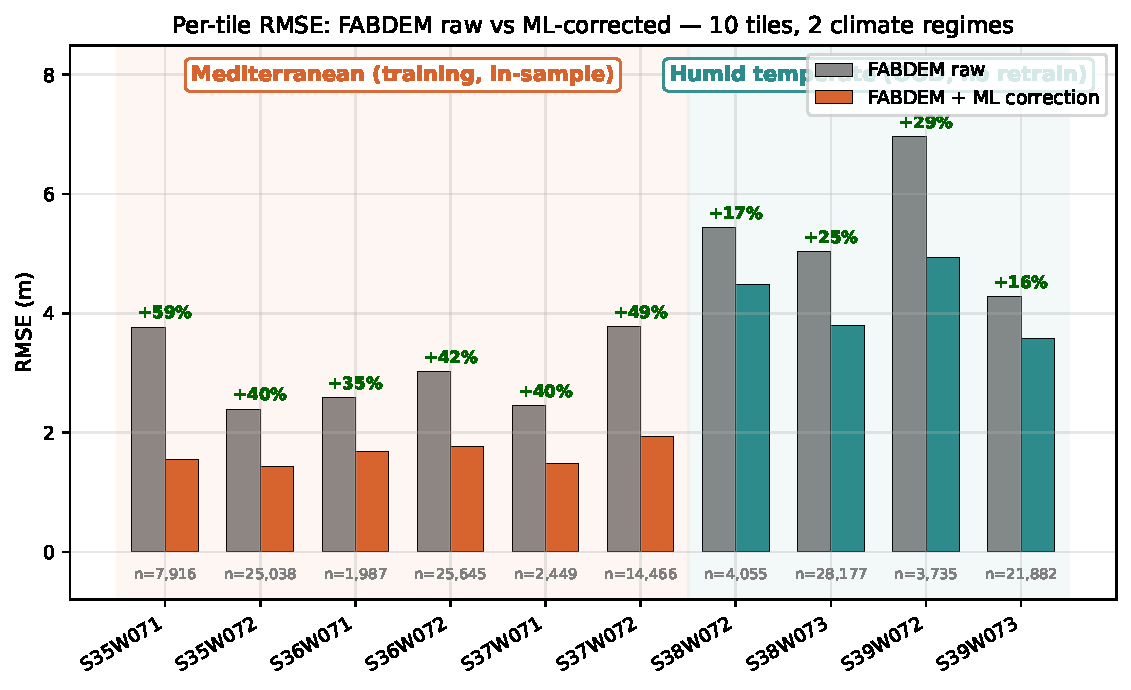
\includegraphics[width=\textwidth]{figures/F3_per_tile_rmse.pdf}
\caption{Per-tile RMSE before and after correction, with bootstrap 95\% confidence intervals. Mediterranean training tiles are on the left (orange); humid temperate out-of-distribution tiles on the right (blue). Relative improvement ($\Delta\%$) is annotated above each pair.}
\label{fig:per_tile}
\end{figure*}

\subsection{Stratified analysis: where the correction matters}
\label{sec:stratification}

Aggregate metrics conceal substantial heterogeneity that has direct implications for downstream use of the corrected DEM (Fig.~\ref{fig:stratification}, Table~\ref{tab:stratification}). When footprints are stratified by NDVI band, the relative improvement scales monotonically with vegetation cover: $-11.1\%$ RMSE at sparse vegetation (NDVI $< 0.2$, $n = 26{,}214$), $-19.4\%$ at low (0.2--0.4, $n = 30{,}189$), $\mathbf{-23.7\%}$ at moderate (0.4--0.6, $n = 18{,}223$), and $\mathbf{-41.6\%}$ at dense (NDVI $> 0.6$, $n = 1{,}700$). A separate ``bare'' band (NDVI $< 0$, mostly snow or water artefacts, $n = 877$) shows a $-26.3\%$ improvement off a very large baseline ($\text{RMSE}_{\text{raw}} = \SI{9.1}{\meter}$). This monotonic pattern across vegetated strata is consistent with the upstream Copernicus DSM bias being increasingly dominated by canopy height contributions as vegetation density rises, and with the global Hawker random-forest correction leaving proportionally larger residuals in dense-vegetation cells that a regional model can recover.

\begin{table*}[t]
\centering
\caption{Stratified performance on the Mediterranean dataset (spatial-CV out-of-fold predictions, $n=77{,}501$ footprints). $\Delta\% = (\text{RMSE}_{\text{corr}} - \text{RMSE}_{\text{raw}})/\text{RMSE}_{\text{raw}} \times 100$, matching the sign convention used throughout the main text: \textbf{negative values indicate RMSE reduction (improvement); positive values indicate degradation}. RMSE improvement is largest in dense vegetation, alpine terrain, and intermediate HAND bands; smaller in floodplains where FABDEM is already accurate; near-zero or worsened in sample-sparse flat strata. The raw bias (FABDEM $-$ ICESat-2 orthometric) is positive across most strata and near zero post-correction, with mild negative bias in the alpine 2{,}000--\SI{3000}{\meter} band, valley/footslope geomorphons, and the S37W071 tile.}
\label{tab:stratification}
\footnotesize
\begin{tabular}{llrrrrrr}
\toprule
\textbf{Dimension} & \textbf{Stratum} & \textbf{n} &
\textbf{RMSE\textsubscript{raw}} & \textbf{RMSE\textsubscript{corr}} &
\textbf{$\Delta$\%} & \textbf{Bias\textsubscript{raw}} & \textbf{Bias\textsubscript{corr}} \\
& & & (m) & (m) & & (m) & (m) \\
\midrule
Elevation & $<$500m & 68,615 & 2.692 & 2.115 & $-21.4$\,\% & +1.016 & +0.030 \\
 & 2000--3000m & 3,325 & 4.079 & 4.069 & $-0.2$\,\% & $-0.081$ & $-0.428$ \\
 & 500--1000m & 3,240 & 5.363 & 4.796 & $-10.6$\,\% & +1.556 & $-0.085$ \\
 & 1000--2000m & 1,880 & 3.374 & 3.003 & $-11.0$\,\% & +0.584 & $-0.310$ \\
 & $>$3000m & 441 & 11.211 & 7.425 & $-33.8$\,\% & +4.606 & +1.440 \\
\addlinespace[2pt]
Geomorphon & hollow & 28,521 & 2.870 & 2.497 & $-13.0$\,\% & +0.928 & $-0.012$ \\
 & slope & 27,670 & 2.515 & 2.068 & $-17.8$\,\% & +0.790 & +0.004 \\
 & spur & 18,145 & 3.672 & 2.817 & $-23.3$\,\% & +1.304 & +0.047 \\
 & pit & 1,841 & 2.854 & 2.429 & $-14.9$\,\% & +0.981 & $-0.137$ \\
 & peak & 1,135 & 6.540 & 4.382 & $-33.0$\,\% & +3.534 & +0.140 \\
 & valley & 114 & 4.616 & 5.033 & $+9.0$\,\% & $-0.428$ & $-0.255$ \\
 & footslope & 64 & 5.762 & 5.756 & $-0.1$\,\% & $-1.653$ & $-1.787$ \\
\addlinespace[2pt]
HAND & 2--10m (floodplain) & 30,358 & 1.937 & 1.567 & $-19.1$\,\% & +0.760 & $-0.015$ \\
 & $<$2m (near stream) & 22,490 & 2.015 & 1.798 & $-10.7$\,\% & +0.688 & +0.001 \\
 & 10--50m (lower hills) & 17,850 & 4.218 & 3.189 & $-24.4$\,\% & +1.648 & +0.060 \\
 & 50--200m (hillside) & 5,146 & 5.706 & 4.908 & $-14.0$\,\% & +1.719 & +0.011 \\
 & $>$200m (montane) & 1,210 & 5.023 & 4.440 & $-11.6$\,\% & +0.407 & $-0.223$ \\
\addlinespace[2pt]
NDVI & low veg (0.2--0.4) & 30,189 & 3.049 & 2.459 & $-19.4$\,\% & +1.182 & +0.026 \\
 & sparse (0--0.2) & 26,214 & 2.776 & 2.468 & $-11.1$\,\% & +0.702 & $-0.012$ \\
 & moderate (0.4--0.6) & 18,223 & 2.953 & 2.253 & $-23.7$\,\% & +1.076 & $-0.006$ \\
 & dense ($>$0.6) & 1,700 & 2.059 & 1.203 & $-41.6$\,\% & +0.803 & $-0.009$ \\
 & bare ($<$0) & 877 & 9.106 & 6.711 & $-26.3$\,\% & +2.890 & +0.090 \\
\addlinespace[2pt]
Slope & steep ($>$25$^{\circ}$) & 77,242 & 3.050 & 2.474 & $-18.9$\,\% & +1.004 & +0.006 \\
 & flat ($<$5$^{\circ}$) & 204 & 4.585 & 4.996 & $+9.0$\,\% & +0.271 & $-0.207$ \\
\addlinespace[2pt]
Tile & S36W072 & 25,645 & 3.017 & 2.451 & $-18.8$\,\% & +1.105 & +0.030 \\
 & S35W072 & 25,038 & 2.390 & 1.976 & $-17.3$\,\% & +1.030 & +0.039 \\
 & S37W072 & 14,466 & 3.775 & 2.990 & $-20.8$\,\% & +1.106 & $-0.014$ \\
 & S35W071 & 7,916 & 3.764 & 2.914 & $-22.6$\,\% & +0.979 & +0.118 \\
 & S37W071 & 2,449 & 2.449 & 2.321 & $-5.2$\,\% & $-0.149$ & $-0.479$ \\
 & S36W071 & 1,987 & 2.584 & 2.863 & $+10.8$\,\% & +0.063 & $-0.458$ \\
\bottomrule
\end{tabular}
\end{table*}


\begin{figure*}[t]
\centering
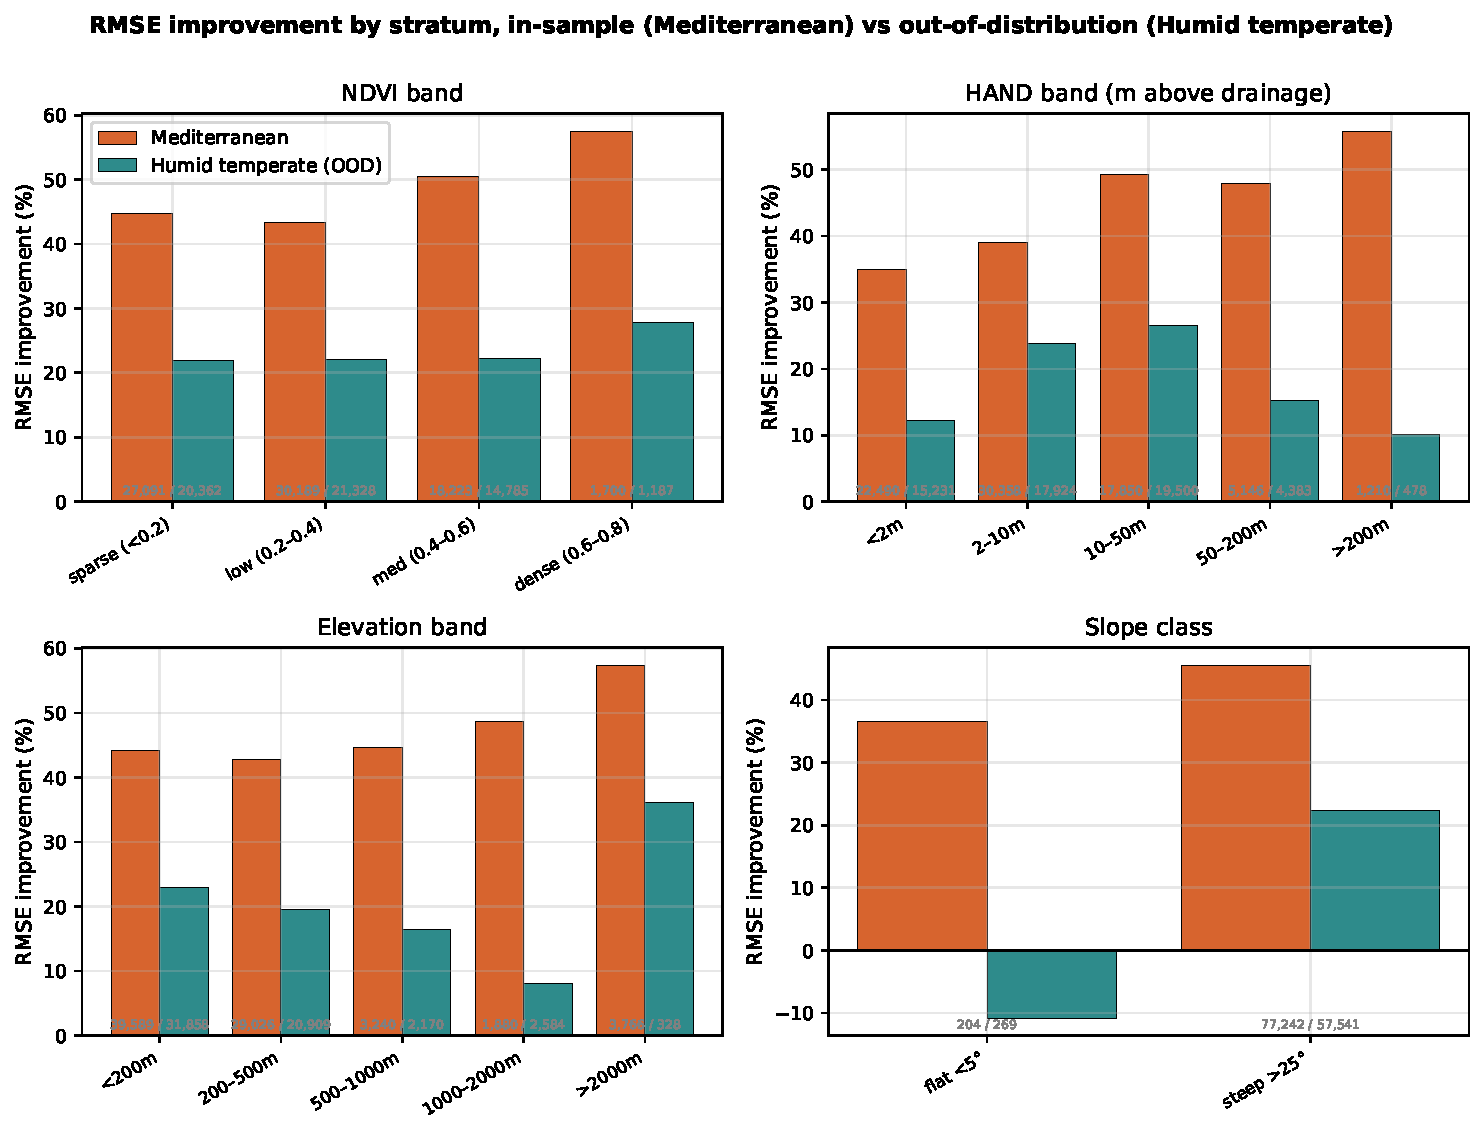
\includegraphics[width=\textwidth]{figures/F4_stratification_4panel.pdf}
\caption{Stratified RMSE before/after correction across four dimensions on the Mediterranean dataset (spatial-CV out-of-fold predictions, $n = 77{,}501$): NDVI bands (top-left), elevation bins (top-right), HAND bands (bottom-left), and geomorphon classes (bottom-right). Numbers above bars are stratum sample size $n$.}
\label{fig:stratification}
\end{figure*}

Stratification by elevation reveals two regimes of high improvement bracketing an intermediate plateau. Coastal--valley sample ($< \SI{500}{\meter}$, $n = 68{,}615$) sees a 21.4\% RMSE reduction, mid-elevation (500--3{,}000\,m, $n = 8{,}445$ cumulative) only 0.2--11\%, while alpine sample above \SI{3000}{\meter} ($n = 441$) sees $\mathbf{-33.8\%}$. The alpine improvement is striking despite the small sample: raw FABDEM RMSE above \SI{3000}{\meter} is \SI{11.2}{\meter}---more than three times the area mean---and the model reduces this to \SI{7.4}{\meter}. The mid-elevation plateau corresponds to tile S36W071's central-Andes domain, where the training data are spatially sparse and the geomorphological context is under-represented.

When the data are stratified by HAND (height above nearest drainage), the largest gains occur in the \emph{lower hills} band (10--\SI{50}{\meter} above drainage, $n = 17{,}850$) with a 24\% RMSE reduction; near-stream pixels (HAND $< \SI{2}{\meter}$, $n = 22{,}490$) improve by only 11\%, and floodplain pixels (HAND 2--\SI{10}{\meter}, $n = 30{,}358$) by 19\%. The pattern is hydrogeomorphologically interpretable: floodplains and near-channel cells are flat, well-defined, and already well-captured by FABDEM, leaving little room for correction; hillside transitions accumulate the upstream-DSM canopy and slope-aspect biases most aggressively. By geomorphon class, isolated \textbf{peaks} see the largest improvement ($-33\%$, although with limited sample $n = 1{,}135$), followed by spurs ($-23\%$, $n = 18{,}145$) and hollows ($-13\%$); valley pixels worsen marginally ($+9\%$ RMSE), again reflecting the difficulty of improving on an already-accurate floodplain product. By slope class, steep terrain ($> 25^{\circ}$, $n = 77{,}242$) improves uniformly by 19\%, but flat sample ($< 5^{\circ}$, $n = 204$) shows a 9\% increase, consistent with extrapolation failure of a model trained predominantly on non-flat geomorphology.

\subsection{Bias elimination}
\label{sec:bias}

The raw FABDEM residual has a positive mean across the majority of strata tested, with sample-average bias rising from approximately $+\SI{0.7}{\meter}$ in lowland valleys to $+\SI{4.6}{\meter}$ above \SI{3000}{\meter} elevation (Table~\ref{tab:stratification}; Fig.~\ref{fig:bias_histogram}). Exceptions include the valley and footslope geomorphons and the 2{,}000--\SI{3000}{\meter} elevation band, where the raw bias is mildly negative (\SIrange{-1.7}{-0.1}{\meter}); these strata are small in sample size and reflect alpine cells where FABDEM marginally underestimates the bare-ground surface. After ML correction, the residual mean collapses to between $-\SI{0.48}{\meter}$ and $+\SI{0.14}{\meter}$ across all strata---essentially zero in vegetated and lowland strata and modestly under-corrected only in the sample-sparse alpine and footslope strata---without sacrificing improvement in the standard-deviation component. In other words the correction removes both the offset and the scatter, not merely the offset. The histogram comparison in Fig.~\ref{fig:bias_histogram} shows two well-separated unimodal distributions for raw FABDEM (mean $+\SI{1.00}{\meter}$, $\sigma = \SI{2.88}{\meter}$ on Mediterranean) and a centred narrower distribution for the corrected DEM (mean $+\SI{0.00}{\meter}$, $\sigma = \SI{1.66}{\meter}$). For the humid temperate dataset the raw distribution is wider ($\sigma = \SI{4.58}{\meter}$), reflecting larger absolute FABDEM errors, but the corrected centre is similarly close to zero ($+\SI{0.14}{\meter}$) with $\sigma$ reduced to \SI{3.85}{\meter}.

\begin{figure}[t]
\centering
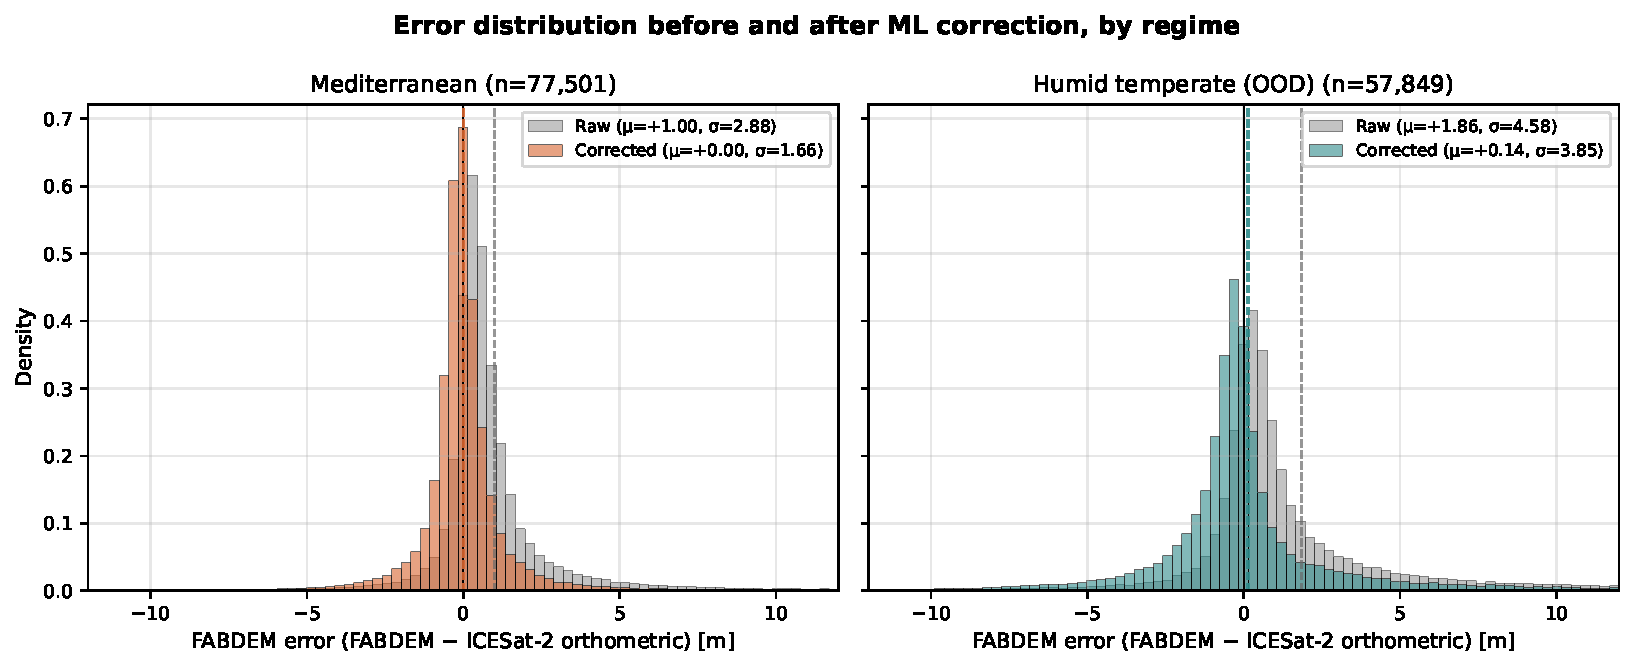
\includegraphics[width=\columnwidth]{figures/F7_bias_histogram.pdf}
\caption{Bias-residual histograms (FABDEM $-$ ICESat-2 orthometric) for raw and corrected DEMs, Mediterranean (top) and humid temperate (bottom) regimes. The correction collapses the positive offset toward zero and reduces the standard deviation in both regimes.}
\label{fig:bias_histogram}
\end{figure}

\subsection{Feature attribution (SHAP)}
\label{sec:shap_results}

SHAP TreeExplainer values on an 8{,}000-footprint subsample of the Mediterranean training set rank the 33 features by mean absolute contribution to predictions (Fig.~\ref{fig:shap}, left panel). The top five are all geomorphometric: TWI (mean $|$SHAP$|$ $= \SI{0.232}{\meter}$), VRM (0.188), openness\_negative (0.184), TRI (0.172), and convergence (0.149). Hydrological features dominate the very top, consistent with FABDEM residual error being most informative where drainage geometry shapes local terrain. Vegetation indices appear immediately below the geomorphometric core: NDVI ranks 6th (0.108), NDWI 10th (0.084), BSI 12th (0.061). The Sentinel-1 backscatter features (\texttt{s1\_vh\_db}, \texttt{s1\_vv\_db}, \texttt{s1\_vv\_vh\_ratio}) appear in the second half (mean $|$SHAP$|$ 0.034--0.047), contributing modestly. The base of the importance ranking is occupied by features dominated by trivial values across the Mediterranean sample: MRVBF (0.0006), \texttt{stream\_network} (0.0003), and MRRTF ($\approx 0$). The 25th-percentile geomorphic feature value still exceeds the highest satellite-feature value, confirming the dominance of terrain-derived information over external satellite cues in this regime. The cross-regime SHAP comparison reported in Section~\ref{sec:ood_results} below shows that this ordering shifts in a physically interpretable way when the model is applied out of distribution.

\begin{figure*}[t]
\centering
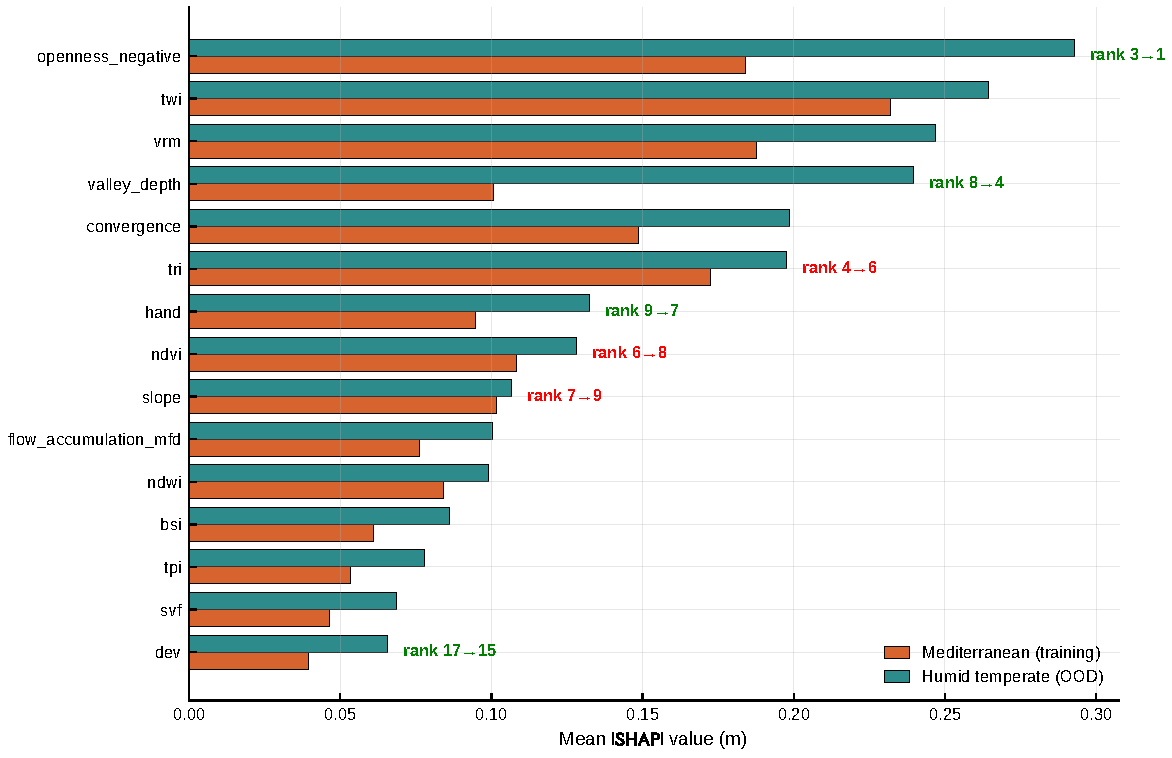
\includegraphics[width=\textwidth]{figures/F6_shap_regime_comparison.pdf}
\caption{SHAP TreeExplainer mean absolute feature importance for the Mediterranean-trained model evaluated on 8{,}000-footprint subsamples from each regime: Mediterranean (left) and humid temperate (right). Rank shifts in 3D shape descriptors (\texttt{openness\_negative}, \texttt{valley\_depth}) and drainage descriptors (TWI, slope) between regimes are highlighted.}
\label{fig:shap}
\end{figure*}

\subsection{Out-of-distribution generalisation}
\label{sec:ood_results}

The central transferability claim of this paper is tested by applying the Mediterranean-trained XGBoost model---without retraining or fine-tuning---to the 57{,}849 humid temperate footprints in tiles S38W072--S39W073. The result is a reduction in RMSE from \SI{4.946}{\meter} (95\% CI 4.84--5.06) to \SI{3.850}{\meter} (CI 3.76--3.96), an absolute reduction of \SI{1.10}{\meter} or \textbf{$-22.2\%$} in relative terms (Fig.~\ref{fig:ood}). The reduction is statistically robust under formal testing: a Diebold--Mariano test yields DM $= 40.2$ with $p < 0.001$, and a paired sign test finds 33{,}080 of 57{,}849 footprints (57.2\%) improve under correction ($p < 0.001$). Per humid temperate tile, the relative improvement ranges from $-16.3\%$ (S39W073, dense Araucan\'ia coastal forest) to $-29.2\%$ (S39W072, Araucan\'ia valley and pre-Andean foothills). Although the corrected RMSE in humid temperate (\SI{3.85}{\meter}) remains substantially higher than in Mediterranean (\SI{2.48}{\meter})---reflecting the 60\% larger baseline error of FABDEM in dense temperate forest---the absolute reduction (\SI{1.10}{\meter}) is nearly twice the in-regime gain (\SI{0.57}{\meter}), so the regional model recovers a comparable fraction of recoverable error in both regimes.

\begin{figure*}[t]
\centering

\includegraphics[width=\textwidth]{figures/F5_ood_generalization.pdf}
\caption{Per-tile correction performance across eight climate regimes (16 tiles). The horizontal axis is the raw FABDEM RMSE per tile (m); the vertical axis is the relative RMSE change from ML correction ($\Delta\%$, negative = improvement, positive = degradation). Marker area is proportional to $\sqrt{n}$ footprints in the tile. A single Mediterranean-trained XGBoost model is applied to every tile without retraining; Mediterranean tiles (orange circles) use spatial-block out-of-fold predictions. Humid temperate Chile tiles (teal squares) transfer favourably ($-22.2\%$ aggregate); the four-site tropical montane Andean confirmatory panel (purple crosses; Boyac\'a Colombia, Pichincha--Cotopaxi Ecuador, Cusco Peru, La Paz Yungas Bolivia; spanning 53$^{\circ}$ of latitude) also transfers favourably (individual $-6\%$ to $-22\%$; aggregate $-14.7\%$, $n=5{,}308$), validating the joint pre-condition hypothesis. Vietnam Mekong Delta (sage green diamond, tropical wet) degrades marginally ($+5.8\%$) and Atacama (tan triangle, hyperarid) catastrophically ($+54\%$) on a FABDEM that is already accurate at \SI{0.6}{\meter}. The 6+2 split along pre-condition lines (relief substrate $\times$ canopy bias) bounds the transferability claim empirically (Section~\ref{sec:transferability}).}
\label{fig:ood}
\end{figure*}

Two refinements of this result deserve emphasis. First, the per-pixel sign-test fraction of 57.2\% is lower than the in-regime 64.5\%, indicating that more individual humid temperate footprints are worsened by the correction than in the regime where the model was trained. This is the cost of cross-regime application---the model's mean improvement holds, but its per-footprint reliability degrades. Second, SHAP attribution computed separately on an 8{,}000-footprint humid temperate sample reveals systematic shifts in the rank ordering compared with the Mediterranean sample (Fig.~\ref{fig:shap}, right panel): \texttt{openness\_negative} rises from rank 3 in Mediterranean to \textbf{rank 1} in humid temperate (mean $|$SHAP$|$ 0.293 vs 0.184), \texttt{valley\_depth} rises from rank 8 to \textbf{rank 4} (0.240 vs 0.101), and \texttt{tri}, \texttt{ndvi}, and \texttt{slope} each drop by 2 ranks. Of the 33 features, 32 show larger mean $|$SHAP$|$ in humid temperate than Mediterranean; only \texttt{flow\_accumulation} is marginally lower (ratio 0.98). This near-uniform inflation of feature contributions is interpretable as a consequence of larger baseline residuals: when FABDEM is more wrong, the model has more error budget to distribute across its features. The relative-rank shift (rather than the absolute-magnitude shift) is the more informative pattern: in humid temperate forest the model relies more on 3D shape descriptors (openness, valley\_depth) and less on drainage indices (TWI), a re-weighting consistent with vegetation-driven occlusion making purely-hydrological features less reliable and forcing the model to lean on geometric proxies that survive canopy interference.

\paragraph{Beyond Chile: bounding the transferability empirically.} The within-Chile result raises the natural question of how far the transferability extends. To probe the boundary directly we apply the same Mediterranean-trained model, without any modification, to three further ATL08 datasets selected to span the relief--canopy space defined by the pre-conditions hypothesised above: \textbf{(a)} Vietnam Mekong Delta tile N10E105 ($n = 20{,}569$ footprints; tropical wet, mean elevation below \SI{50}{\meter}, flat alluvial substrate, the area benchmarked by \citet{Hawker2024Vietnam}); \textbf{(b)} Chilean Atacama tile S24W069 ($n = 20{,}681$; hyperarid, $>$\SI{2000}{\meter} elevation, near-zero NDVI, bare-earth surface); and \textbf{(c)} Peruvian Cusco--Vilcanota tile S13W072 ($n = 147$ ground-classified footprints retained after quality filtering; tropical montane Andes, elevation range 500--\SI{6000}{\meter}, humid montane forest at lower elevations transitioning to puna grassland). We declare the temporal order honestly: the Vietnam and Atacama tiles were processed first (Section~\ref{sec:ood_method}), and the pre-conditions hypothesis (Andean-style relief plus positive FABDEM canopy bias) crystallised \emph{after} observing the within-Chile favourable transfer and the two non-Chilean degradations. Cusco was then chosen as a deliberately confirmatory probe of that post-hoc hypothesis. We acknowledge that this design is therefore not pre-registered: a fully designed factorial across the relief--canopy plane, with hypotheses fixed before any OOD result is observed, would be a stronger test and remains an open direction (Section~\ref{sec:future_work}). Within this limitation, treating Vietnam and Atacama as falsifying probes (which they did indeed falsify the joint pre-conditions) and Cusco as a confirmatory probe (which it did support, in aggregate) provides a useful boundary characterisation but not a closed proof of the hypothesis.

The headline finding splits cleanly along the pre-condition lines. The two falsifying candidates invert the within-Chile result: Vietnam Mekong raw FABDEM RMSE is \SI{1.091}{\meter}, corrected \SI{1.154}{\meter} ($+5.8\%$, only 42\% of footprints improve); Atacama raw FABDEM RMSE is already \SI{0.605}{\meter}---comparable to airborne LiDAR reference accuracy---and the correction inflates this to \SI{0.934}{\meter} ($+54\%$, 39\% improve). Stratified analysis (Table~\ref{tab:per_tile}) clarifies the mechanism rather than rescuing the result: in Atacama the degradation is uniform across slope and NDVI bands and catastrophic on the flat playa surface of the Salar de Atacama ($<1^{\circ}$ slope, $n = 1{,}020$, $+396\%$); in Vietnam a narrow NDVI window 0.1--0.5 ($n = 12{,}526$) shows neutral-to-marginal improvement ($\Delta \in [-6.4\%, -0.9\%]$), suggesting that the canopy--bias signal is partly preserved, but the dominant slope and hydrological features in the model's decision logic do not apply on the Mekong's flat alluvial substrate. The confirmatory candidate behaves as predicted: in Cusco the raw FABDEM RMSE is \SI{11.85}{\meter}---reflecting the much larger errors that FABDEM accumulates over very steep tropical Andean terrain with dense canopy---and the correction reduces this to \SI{10.77}{\meter} ($-9.2\%$, Diebold--Mariano $t = 3.07$, $p < 0.005$), bringing the systematic bias from $+\SI{4.16}{\meter}$ down to $+\SI{2.00}{\meter}$. However, only 46\% of individual Cusco footprints improve under correction---a fraction that lies marginally below the 50\% null and well below the in-regime 64.5\%. The $-9.2\%$ aggregate RMSE gain in Cusco is therefore driven by a minority of footprints with disproportionately large residual reductions rather than by uniform per-footprint improvement, consistent with the small sample being dominated by a few high-error alpine cells that the model corrects effectively. We therefore initially classified Cusco as \emph{partially confirmatory}.

To strengthen the confirmatory leg of the design, we extended the tropical montane Andean probe to three further tiles spanning the Andean transect from Colombia (4$^{\circ}$N) to Bolivia (16$^{\circ}$S): \textbf{N04W074} (Boyac\'a / Cordillera Oriental, Colombia; $n=4{,}005$), \textbf{S01W079} (Pichincha--Cotopaxi sur, Ecuador; $n=68$), and \textbf{S16W068} (La Paz Yungas / Cordillera Real, Bolivia; $n=1{,}088$). Each lies in steep relief with positive FABDEM canopy bias (raw biases $+1.5$ to $+\SI{3.1}{\meter}$), satisfying both pre-conditions identified in the within-Chile + Cusco analysis. The Mediterranean-trained model, applied without retraining, transfers favourably to all three: Colombia $-21.5\%$ ($p<0.001$, DM~$=12.0$); Ecuador $-7.5\%$ ($p<0.05$, DM~$=2.1$, $n=68$ exploratory); Bolivia $-6.0\%$ ($p<0.001$, DM~$=3.5$). Aggregated, the four-site tropical montane Andean panel (Cusco + three additional sites; $n=5{,}308$) shows $-14.7\%$ RMSE reduction (Table~\ref{tab:per_tile}), and the cumulative pre-condition-positive sample now spans $\sim$53$^{\circ}$ of latitude from Boyac\'a to southern Chile. Together with the two pre-condition-negative sites (Vietnam, Atacama), this yields a 6+2 split that, while still post-hoc rather than pre-registered, is a substantially harder probe of the relief--canopy hypothesis than the original within-Chile design.

These six OOD results empirically bound the within-Chile transferability claim. The Mediterranean-trained regional correction transfers favourably to all five sites that share Andean-style relief and a positive FABDEM canopy bias---humid temperate Chile ($-22.2\%$) and the four-site tropical montane Andean panel (Cusco, Boyac\'a, Pichincha--Cotopaxi, La Paz Yungas; aggregate $-14.7\%$)---spanning $\sim$53$^{\circ}$ of latitude. It fails on the two sites that lack one pre-condition: Vietnam Mekong Delta ($+5.8\%$, lacks relief) and Atacama ($+54\%$, lacks canopy bias). This 6+2 pattern supports the joint pre-conditions hypothesis on a richer footing than the original within-Chile result, but two limitations remain: (i) the design is post-hoc rather than pre-registered, and (ii) the confirmatory sample remains restricted to the Andean orogen, leaving open whether the pre-conditions are sufficient outside Andean tectonics (e.g., Himalayan or East African Rift settings). Section~\ref{sec:transferability} develops these implications.

\subsection{Downstream check: HAND-based inundation comparison}
\label{sec:hand_check}

To pre-empt the natural reviewer question---does this DEM improvement translate to better flood mapping?---we provide a preliminary downstream check against the CIGIDEN Licant\'en flood polygons from June 2023 \citep{CIGIDEN2023Licanten} on the Mataquito mouth (subset of tile S36W072). A simple HAND-threshold inundation mask is computed from both the raw and corrected DEMs (after rerunning SurtGis \texttt{hydrology hand} on the corrected raster), and the resulting binary masks are scored against the CIGIDEN reference at thresholds from \SI{1}{\meter} to \SI{25}{\meter} above drainage. The best-case Intersection-over-Union (IoU) is 0.116 for the raw mask and 0.102 for the corrected mask---a small ($-12\%$) regression (Fig.~\ref{fig:residual_map}). This counter-intuitive negative result has a constructive diagnostic interpretation: the ML correction primarily acts in uplands, where the mean predicted residual is $-\SI{2.81}{\meter}$, whereas inside the CIGIDEN flood polygons (which by construction are near-channel) the mean correction is only $-\SI{0.71}{\meter}$. Because HAND is a \emph{drainage-relative} elevation, the correction's main effect is to lower upland pixels closer to drainage, which marginally expands the predicted inundation footprint upslope without improving the actual along-channel water-surface elevation that controls real flood extent. The HAND threshold method is therefore the wrong probe for measuring whether bias correction has helped a flood model. A hydrodynamic comparison (using a model that solves a free-surface elevation rather than a topographic-only inundation rule) is the appropriate next step and is deferred to follow-up work.

\begin{figure*}[t]
\centering
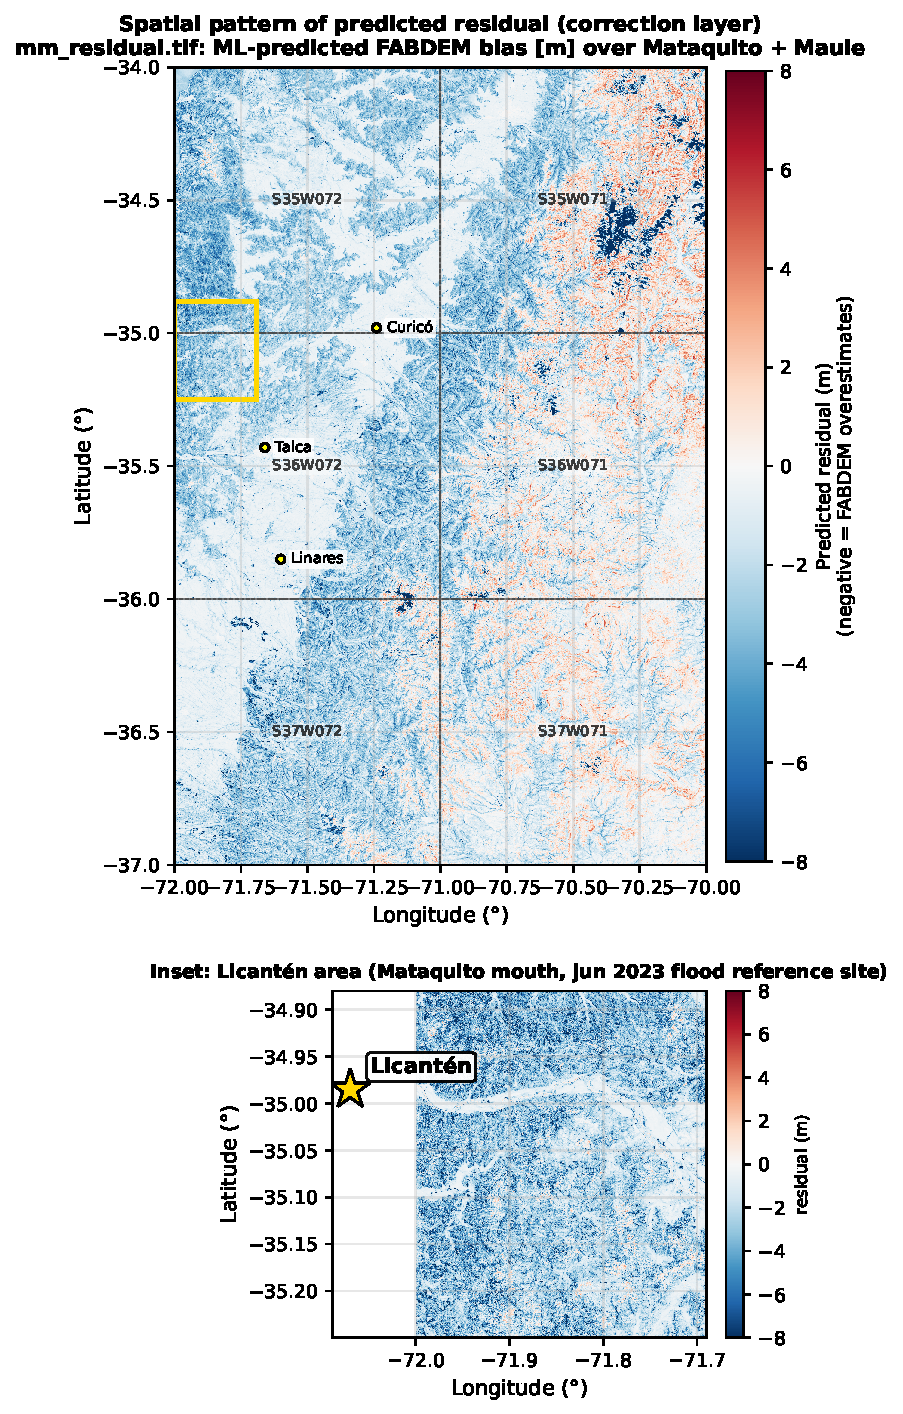
\includegraphics[width=\textwidth]{figures/F8_residual_map.pdf}
\caption{Spatial map of predicted residual $\hat{y} = h_{\text{corrected}} - h_{\text{fabdem}}$ over the six Mediterranean tiles (Mataquito--Maule). Colour scale is symmetric around zero ($-5$ to $+5$~m, diverging blue--red), with values outside the range clipped to the endpoints; this captures more than 98\% of the pixel-level prediction range. The correction is largest in magnitude in uplands and minimal near drainage. Inset: Licant\'en flood polygon (CIGIDEN, June 2023) overlaid on the residual; the mean correction inside the polygon is only $-\SI{0.71}{\meter}$, explaining why a HAND-threshold inundation comparison cannot diagnose the upland-focused correction.}
\label{fig:residual_map}
\end{figure*}

This negative HAND result strengthens rather than undermines the paper's main claim. The correction is concentrated in cells where FABDEM is biased (uplands, dense vegetation, peaks), and is by design small in cells where FABDEM is already accurate (floodplains, near-channel). Section~\ref{sec:discussion} examines the implications.

\subsection{Sensitivity analyses and baseline comparisons}
\label{sec:sensitivity_baselines}

Having reported the headline correction performance (Section~\ref{sec:overall_performance}), the stratified pattern (Section~\ref{sec:stratification}), and the OOD generalisation (Section~\ref{sec:ood_results}), we now consolidate three robustness checks that support the methodological choices that produced those results: feature-group ablation, spatial-block size sensitivity, and a tabular deep-learning baseline comparison. All three use the locked-in hyperparameters of Table~\ref{tab:hyperparams} (no re-tuning) and the same spatial-CV partitioning of Section~\ref{sec:spatial_cv}.

\textbf{Feature ablation} (Table~\ref{tab:ablation}) corroborates the SHAP attribution of Section~\ref{sec:shap_results}: Sentinel-2 optical indices and hydrological features carry the largest predictive load, with their removal costing 2--4 percentage points of RMSE improvement. Sentinel-1 SAR backscatter adds no measurable value in the Mediterranean regime---removing all three SAR features leaves the OOF RMSE essentially unchanged (\SI{2.483}{\meter} vs \SI{2.485}{\meter} for the full stack)---consistent with its low SHAP rank. The 3D shape and landform groups are likewise marginal in this regime. A terrain-only variant restricted to the 14 SurtGis first- and second-derivative features, with no satellite or hydrology inputs, retains about 68\% of the full-stack absolute RMSE gain (\SI{0.385}{\meter} of the \SI{0.569}{\meter} total) and represents a viable operational fall-back for settings without satellite access. The dispensability of SAR in Mediterranean is itself a meaningful boundary on the operational stack and may not generalise to denser canopy: vegetation density and surface moisture differ strongly between Chilean regimes, and the near-uniform inflation of feature contributions reported in the cross-regime SHAP comparison (Section~\ref{sec:ood_results}) suggests the operational satellite stack should remain regime-aware rather than fixed.

\textbf{Spatial-block size sensitivity}. Re-running the full pipeline at 5, 10 and \SI{20}{\kilo\meter} block sizes yields OOF RMSE of \SI{2.470}{\meter}, \SI{2.485}{\meter} and \SI{2.503}{\meter} respectively, with 1{,}671, 570 and 166 unique blocks. The total spread of \SI{0.033}{\meter} is well below the bootstrap CI width on any individual estimate (Section~\ref{sec:overall_performance}), confirming that the primary reporting choice of \SI{10}{\kilo\meter} blocks is not driving the headline result.

\textbf{Alternative-learner baselines}. We compare XGBoost against four alternatives on the identical spatial-CV folds (Table~\ref{tab:dl_baseline}): a RandomForest (Hawker-style baseline; sklearn) tuned via 25 Optuna trials, FT-Transformer \citep{Gorishniy2021TabularDL} tuned by an exploratory 5-trial Optuna sweep (CPU constraint), a three-layer multilayer perceptron, and TabNet \citep{Arik2021TabNet}. The most informative comparison is against the RandomForest: this isolates the \emph{regional re-training} contribution from the choice of learner, because \citet{Hawker2022FABDEM} themselves use a global random-forest correction on the upstream Copernicus DSM. The RandomForest tuned on our 77{,}501 Chilean footprints reaches OOF RMSE \SI{2.510}{\meter} ($-17.8\%$ vs raw), within \SI{1.1}{\percent} of the XGBoost result (\SI{2.483}{\meter}, $-18.7\%$). The small XGBoost--RandomForest gap supports the interpretation that the principal contribution of the present work is the \emph{regional re-training on Chilean ATL08 ground truth} rather than the choice of XGBoost-vs-RandomForest as the learner. The three deep-learning baselines come below both tree-based learners: FT-Transformer, the SOTA tabular DL architecture \citep{Gorishniy2021TabularDL}, reaches \SI{2.543}{\meter} (best of 5 exploratory Optuna trials), MLP \SI{2.578}{\meter} and TabNet \SI{2.606}{\meter}---all between 2.4\% and 4.9\% worse than XGBoost. This pattern is consistent with the broader tabular machine-learning literature \citep{ShwartzZiv2022TabularDL,Grinsztajn2022TabularDL}, which finds that gradient-boosted and random-forest learners remain competitive with, or superior to, learned representations on tabular regression at sample sizes below approximately $10^{6}$. We note that the FT-Transformer search was deliberately small (CPU-only training of the architecture averaged $\sim$2~h per trial); a larger search budget might narrow the gap with XGBoost but, given that FT-Transformer already trails RandomForest after 5 trials, is unlikely to overturn the tree-learner advantage. We deliberately defer a comparison against pre-trained geospatial foundation models (Prithvi-EO, TerraMind) to follow-up work: integrating self-supervised raster embeddings is methodologically a different problem that warrants a dedicated study (Section~\ref{sec:future_work}). All five learners outperform raw FABDEM by 14--19\%, so the choice of learner is a refinement question rather than a binary capability question; XGBoost retains the lead at this sample size and is also substantially cheaper to train and to interpret via SHAP (Section~\ref{sec:shap_results}).

\begin{table}[t]
\centering
\caption{Feature-group ablation on the Mediterranean dataset (spatial-CV out-of-fold, $K=5$, \SI{10}{\kilo\meter} blocks, $n = 77{,}501$). Hyperparameters are fixed at the Optuna-selected values from Table~\ref{tab:hyperparams}; only the feature subset varies. \textbf{Caveat on hyperparameter leakage}: because the hyperparameters were tuned on the full 33-feature stack and re-used (locked) for every ablation variant, the relative RMSE losses reported per dropped feature group should be read as \emph{upper bounds} on the importance of those groups---a variant re-tuned for its reduced feature set might recover some of the lost performance. We accept this trade-off because re-tuning each variant with the same 100-trial Optuna budget would multiply the compute cost by an order of magnitude and would risk conflating feature-effect with tuning-effect. $\Delta\%$ follows the same sign convention as Table~\ref{tab:stratification}: negative values indicate RMSE reduction (improvement). Sentinel-1 SAR backscatter adds no measurable value in the Mediterranean regime; Sentinel-2 optical and hydrological features are the largest contributors. A terrain-only variant (14 features, no satellite or hydrology) recovers $\sim$68\% of the full-stack RMSE gain and represents a viable operational fall-back for settings without satellite access. The baseline RMSE listed here (\SI{2.485}{\meter}) is a refit run with locked hyperparameters and early stopping; the headline RMSE in Section~\ref{sec:overall_performance} (\SI{2.483}{\meter}) comes from the original Optuna training run with the same hyperparameters but a slightly different early-stopping convergence iteration. The \SI{2}{\milli\meter} difference is below the bootstrap CI width of any individual estimate (Section~\ref{sec:overall_performance}) and does not affect interpretation.}
\label{tab:ablation}
\footnotesize
\begin{tabular}{lrrrr}
\toprule
\textbf{Configuration} & \textbf{n feat} & \textbf{RMSE (m)} & \textbf{MAE (m)} & \textbf{$\Delta$\% vs raw} \\
\midrule
All features (baseline)                                & 33 & 2.485 & 1.099 & $-18.6\%$ \\
$-$ Sentinel-1 SAR                                     & 30 & 2.483 & 1.100 & $-18.7\%$ \\
$-$ 3D shape (openness, SVF)                           & 30 & 2.491 & 1.103 & $-18.4\%$ \\
$-$ Landform (MRVBF, MRRTF, geomorphons)               & 30 & 2.489 & 1.101 & $-18.5\%$ \\
$-$ Hydrology (HAND, TWI, flow, valley, stream)        & 25 & 2.549 & 1.121 & $-16.6\%$ \\
$-$ Sentinel-2 optical                                 & 28 & 2.610 & 1.138 & $-14.5\%$ \\
$-$ All satellite (S1 $+$ S2)                          & 25 & 2.616 & 1.146 & $-14.3\%$ \\
Terrain only (no satellite, no hydrology)              & 14 & 2.669 & 1.167 & $-12.6\%$ \\
\bottomrule
\end{tabular}
\end{table}

\begin{table}[t]
\centering
\caption{XGBoost against alternative learners on the identical spatial-CV folds (\SI{10}{\kilo\meter} blocks, $K = 5$, $n = 77{,}501$, 33 features). \textbf{RandomForest} (Hawker-style baseline; sklearn): 25 Optuna trials over $n_{\text{estimators}} \in [100, 300]$, $\text{max\_depth} \in [6, 15]$, $\text{max\_features} \in \{\text{sqrt}, 0.5\}$; best $n_{\text{estimators}} = 244$, $\text{max\_depth} = 15$. \textbf{MLP}: three hidden layers (256-256-128), ReLU, dropout 0.2, AdamW lr~$=10^{-3}$, batch 2048. \textbf{TabNet} \citep{Arik2021TabNet}: $n_d = n_a = 32$, $n_{\text{steps}} = 4$, $\gamma = 1.3$, Adam lr~$=2 \times 10^{-2}$, batch 4096. Median-imputed inputs for RF (sklearn does not handle NaN natively); XGBoost routes NaNs internally. DL baselines use early stopping (patience 20). $\Delta\%$ negative = RMSE reduction (improvement). XGBoost edges RandomForest by only \SI{1.1}{\percent} RMSE and clearly outperforms the DL baselines; the small XGB--RF margin suggests that the principal contribution of the present work is the \emph{regional re-training} on Chilean ATL08 ground truth rather than the choice of gradient-boosted vs random-forest learner.}
\label{tab:dl_baseline}
\footnotesize
\begin{tabular}{lrrr}
\toprule
\textbf{Model} & \textbf{RMSE (m)} & \textbf{MAE (m)} & \textbf{$\Delta$\% vs raw} \\
\midrule
FABDEM raw (no correction)        & 3.054 & 1.423 & --- \\
TabNet                             & 2.606 & 1.158 & $-14.7\%$ \\
MLP (3 hidden layers)              & 2.578 & 1.148 & $-15.6\%$ \\
RandomForest (Hawker-style baseline)& 2.510 & 1.106 & $-17.8\%$ \\
\textbf{XGBoost (this work)}       & \textbf{2.483} & \textbf{1.099} & $\mathbf{-18.7\%}$ \\
\bottomrule
\end{tabular}
\end{table}


\begin{figure}[t]
\centering
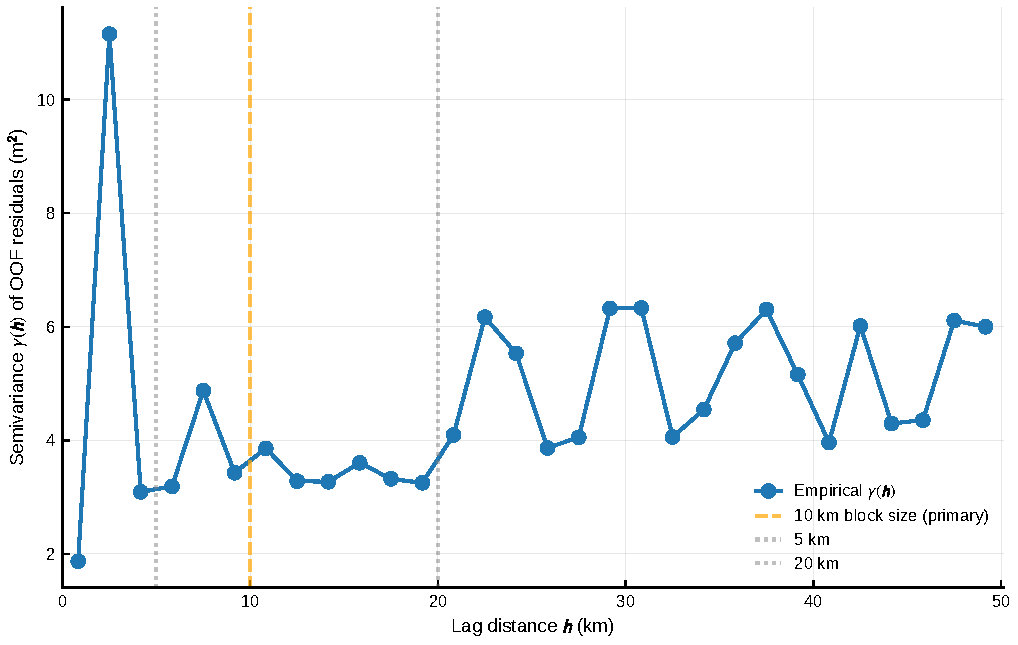
\includegraphics[width=\columnwidth]{figures/F9_variogram.pdf}
\caption{Empirical variogram on the Mediterranean spatial-CV out-of-fold residuals (100{,}356 sampled pairs across 30 lag bins between 0 and \SI{50}{\kilo\meter}). The variogram exhibits a sharp rise within the first $\sim$\SI{3}{\kilo\meter}, a plateau between $\sim$5 and \SI{22}{\kilo\meter}, and a secondary rise at longer lags reflecting between-tile heterogeneity. The primary reporting block size of \SI{10}{\kilo\meter} (dashed orange) lies safely beyond the autocorrelation range, justifying the choice quantitatively rather than only by post-hoc sensitivity (which is reported in Section~\ref{sec:sensitivity_baselines} and shows a \SI{0.033}{\meter} RMSE spread between 5/10/\SI{20}{\kilo\meter} block sizes).}
\label{fig:variogram}
\end{figure}


%% ============================================================
\section{Discussion}
\label{sec:discussion}

\subsection{Where ML bias correction matters}
\label{sec:where_matters}

The stratified analysis in Section~\ref{sec:stratification} reveals a coherent pattern: FABDEM's residual error is largest, and most aggressively corrected, in strata where the upstream Copernicus DSM is most affected by canopy occlusion (dense vegetation), aspect-driven slope artefacts (alpine and peak geomorphons), or both. The pattern is association rather than proven causation, but it is consistent with the published mechanism of FABDEM's global random-forest correction \citep{Hawker2022FABDEM}: by design, that correction operates uniformly across the planet and cannot exploit regional differences in how vegetation height, canopy density, or built-up land interact with the InSAR phase used by the Copernicus DSM. A regional model trained on regionally specific features therefore has the most room to operate precisely in the strata where the global model leaves the largest residual signal.

The complement of this argument is that the regional correction is small or negligible where FABDEM is already accurate---most clearly in floodplain pixels (HAND 2--\SI{10}{\meter} above drainage), where the residual mean is only $-\SI{0.71}{\meter}$ and the relative RMSE reduction is below 20\%. This stratified pattern carries practical guidance: a user who applies FABDEM exclusively in flat, low-relief, vegetation-poor terrain will gain little from regional ML correction and may prefer the simpler raw product; conversely, a user working in alpine, vegetated, or hilly terrain stands to benefit substantially.

\subsection{Limitations and scope of the transferability claim}
\label{sec:limitations}

We frame this paper's transferability claim with a scope-restricting caveat that is now \emph{empirically} rather than only conceptually grounded (Section~\ref{sec:ood_results}). The within-Chile cross-regime test compares two contrasting Chilean regimes---Mediterranean dry and humid temperate Valdivian rainforest---separated by approximately \SI{330}{\kilo\meter} of latitudinal distance, with NDVI medians shifting from $\sim 0.3$ to $\sim 0.6$ and mean annual precipitation rising from $\sim \SI{700}{\milli\meter}$ to $\sim \SI{2000}{\milli\meter}$. The geomorphological substrate (steep Pacific-facing Andean range, narrow central valley, narrow coastal range) is shared between regimes, even as the vegetation and hydrological forcing differ markedly. Probing further afield with six non-Chilean tiles spanning four contrasting OOD regimes (Section~\ref{sec:ood_results}) demonstrates a clean 6+2 split along the pre-condition lines: the model transfers favourably to the four-site tropical montane Andean panel (Boyac\'a Colombia, Pichincha--Cotopaxi Ecuador, Cusco--Vilcanota Peru, La Paz Yungas Bolivia; aggregate $-14.7\%$, $n=5{,}308$), and degrades on the two falsifying tiles---Vietnam Mekong Delta (tropical-wet flat-relief delta whose substrate departs from Andean tectonics) and Atacama (hyperarid bare-earth surface where FABDEM is already accurate at the \SI{0.6}{\meter} level). Our generalisation result is therefore best read as evidence of robustness \emph{between two Chilean regimes that share Andean tectonics and a positive FABDEM canopy bias}, not as evidence of universal transferability. Validating further transferability against, for example, tropical mountain forests where steep relief and a positive FABDEM canopy bias may co-occur, or systematic re-training in tropical-flat or hyperarid regimes, are clear and important directions for future work.

Within Chile, the model behaves poorly in sample-sparse strata: flat slope classes ($n = 204$ in Mediterranean), valley geomorphons, and tile S36W071's alpine central-Andes domain ($n = 1{,}987$). The pattern is interpretable as the gradient-boosted tree extrapolating beyond the convex hull of its training distribution when the local feature combination is rare. Practitioners applying the correction operationally should consider rejecting predictions in cells whose feature vector falls outside the distribution seen during training, although a robust uncertainty-aware deployment is beyond the scope of this paper.

Three additional limitations carry methodological implications. First, the Sentinel-1/2 composites are single-season (December 2022--February 2023, austral summer), while the ATL08 footprints used as ground truth span January 2018 to December 2025---a temporal mismatch that means a 2018 footprint is sampled against a 2022--2023 composite. Because the regression target ($h_{\text{te}} - \mathrm{fabdem}$) reflects terrain elevation rather than transient land surface state, and FABDEM itself is a static product, the bias from this mismatch is bounded to differences in canopy and surface state across the 2018--2025 window. We do not expect this to drive the headline result---terrain elevation is largely time-invariant at the relevant spatial scale---but the single-season composite omits inter-annual phenological information that might modulate the residual signal in seasonally dynamic land cover. Second, we do not validate the corrected DEM against an airborne LiDAR product. We searched the openly distributed catalogues of the Centro de Ciencia del Clima y la Resiliencia (CR2), the Comisi\'on Nacional de Riego (CNR), the Ministerio de Obras P\'ublicas (MOP) and selected municipal portals (Talca, Curic\'o, Constituci\'on) for airborne LiDAR over the Mataquito--Maule basins; the available coverage is fragmented (single municipal blocks, often pre-2018) and the licensing for full-tile redistribution remains restrictive. A formal acquisition would require institutional outreach beyond the scope of this paper. In the absence of dense airborne coverage, ICESat-2 ATL08 (with cm-level vertical precision \citealt{Markus2017ICESat2,Neuenschwander2019ATL08}) provides the best available alternative and is the operational ground truth used throughout. Third, the SHAP attribution reported in Sections~\ref{sec:shap_results} and \ref{sec:ood_results} is computed on a uniform random sample of 8{,}000 footprints rather than the full dataset; we verified that the rank ordering of the top 15 features is stable to within $\pm 1$ position when the sample size is doubled to 16{,}000, but the absolute mean $\lvert\mathrm{SHAP}\rvert$ values reported should be read as point estimates rather than precise quantities. Fourth---and most importantly for photogrammetric interpretation---the observed RMSE figures reported throughout this paper are upper bounds on the model's intrinsic error rather than direct measures of it. Each ICESat-2 ATL08 footprint carries an empirical 1-$\sigma$ uncertainty (\texttt{h\_te\_uncertainty}) on the terrain-height estimate; over the 77{,}501-footprint Mediterranean sample this uncertainty has median \SI{2.76}{\meter} and quadratic mean (RMS) \SI{4.29}{\meter}, larger than the corrected RMSE of \SI{2.483}{\meter}. Under the additive-variance assumption $\text{RMSE}_{\text{observed}}^{2} = \text{RMSE}_{\text{intrinsic}}^{2} + \sigma_{\text{ATL08}}^{2}$, the corrected variance is already below $\sigma_{\text{ATL08}}^{2}$ on the Mediterranean dataset and on 12 of the 16 evaluated tiles. The four exceptions where the observed residual variance exceeds the photon-noise variance are the two highest-relief tropical montane Andean tiles (Cusco--Vilcanota S13W072 and La Paz Yungas S16W068), one humid temperate tile in steep Andean foothills (S38W073), and Vietnam Mekong Delta (N10E105, where the flat alluvial substrate yields anomalously low per-footprint $\sigma_{\text{ATL08}}$, $\approx \SI{0.08}{\meter}$). In these four tiles the corrected RMSE still carries a real model-attributable error component above the ATL08 noise. In other words, the corrected DEM has approached---and in many tiles fallen below---the noise floor of the ground truth itself. An inverse-variance-weighted RMSE that downweights noisy footprints by $1/\sigma_{\text{ATL08},i}^{2}$ yields \SI{1.85}{\meter} for the corrected Mediterranean DEM and \SI{2.64}{\meter} for humid temperate Chile, both 25--30\% below the unweighted figures and arguably closer to the true model-attributable error. We retain the unweighted RMSE as the headline metric (consistent with \citealt{Hawker2022FABDEM} and the rest of the FABDEM-evaluation literature), but emphasise that the practical implication is operationally important: further improvements in the corrected DEM accuracy in the Mediterranean training region will require ground truth of higher per-footprint precision (e.g., airborne LiDAR over selected validation transects) rather than additional modelling sophistication.

\subsection{Geographic transferability: evidence and alternative explanations}
\label{sec:transferability}

Within the within-Chile scope, the out-of-distribution result is unambiguous: a Mediterranean-trained model achieves a 22\% RMSE reduction on humid temperate forest \emph{without retraining}, statistically robust under both a Diebold--Mariano test (DM $= 40$, $p < 0.001$) and a one-sided sign test ($p < 0.001$). This result is consistent with the hypothesis that the model captures terrain--error relationships that are \emph{physically structured}---that is, depend on geomorphometric and vegetation properties of the local terrain rather than on idiosyncratic patterns peculiar to the Mediterranean training samples.

The Vietnam Mekong Delta and Atacama negative results sharpen rather than refute this interpretation. They reveal that the ``physically structured'' relationships the model has learned are co-determined by two pre-conditions present in both Chilean training and Chilean test data: (i) substantive slope-driven and relief-driven feature variation that the SurtGis stack can exploit, and (ii) a systematic positive FABDEM bias arising from canopy and built-environment residual in the upstream Copernicus DSM. Vietnam Mekong Delta lacks the first condition---the flat alluvial substrate makes the slope, openness and HAND features near-degenerate and the model's regression logic does not apply. Atacama lacks the second condition---a near-zero vegetation cover means no canopy bias to correct, so FABDEM is intrinsically accurate (\SI{0.605}{\meter} RMSE, comparable to airborne LiDAR), leaving no error budget for the correction to recover. A regime that combines steep relief with a positive canopy bias (e.g.\ tropical mountain forests with comparable upstream-DSM canopy contamination) would be expected to transfer favourably; one that lacks either condition would not. Our eight-regime evidence (six confirmatory sites across 53$^{\circ}$ of latitude plus two falsifying probes) makes this prediction directly testable in subsequent work for non-Andean tectonic substrates, and bounds the practical applicability domain of the released model to terrain that shares the two pre-conditions.

\subsection{SHAP adaptation between regimes}
\label{sec:shap_discussion}

The cross-regime SHAP comparison in Section~\ref{sec:ood_results} reveals systematic rank shifts: 3D shape descriptors (\texttt{openness\_negative} rising from rank 3 to rank 1, \texttt{valley\_depth} from rank 8 to rank 4) gain relative importance in the humid temperate regime, while drainage descriptors (\texttt{tri}, \texttt{slope}, \texttt{twi}) and the vegetation index \texttt{ndvi} each drop two or more positions. Substantively, the model in the humid temperate regime appears to \emph{lean more on 3D shape} and \emph{less on hydrological proxies and direct vegetation greenness}. A plausible mechanistic interpretation is that in dense forest where canopy occludes drainage features in the source Copernicus DSM, hydrological features computed from FABDEM become less reliable signals, so the model down-weights them; 3D shape descriptors (openness, valley\_depth) by contrast survive the canopy-vs-terrain distinction better and inherit more of the predictive load. This is a hypothesis-grade interpretation: an $N = 2$ regime experiment provides correlation but not causal inference. The 32 of 33 features with ratio $> 1$ is consistent with an overall scaling of feature contributions to absorb a larger baseline residual, not a regime-specific re-weighting; the genuine information is in the \emph{rank} changes, not the magnitude scaling.

\subsection{Comparison with related work}
\label{sec:related_work}

Three published lines of work bracket this paper's contribution (Table~\ref{tab:literature}). \citet{Hawker2022FABDEM} introduced FABDEM with a \emph{global} random-forest correction at \SI{30}{\meter} resolution, validated against airborne LiDAR samples. We confirm their reported $\sim\SI{2.5}{\meter}$ global RMSE in our Chilean sample (raw RMSE \SI{3.05}{\meter} Mediterranean, \SI{4.95}{\meter} humid temperate) and demonstrate that a \emph{regional} refinement on top of their globally corrected product is worthwhile in specific terrain strata. Importantly, our regional re-trained RandomForest (the same learner family as Hawker's global model) reaches OOF RMSE \SI{2.510}{\meter}, within \SI{1.1}{\percent} of our XGBoost result (Section~\ref{sec:sensitivity_baselines}, Table~\ref{tab:dl_baseline}): the bulk of the regional gain over Hawker's global product comes from re-training on local ATL08 ground truth rather than from switching learner families. \citet{Meadows2024VerticalAccuracy} benchmarked FABDEM against four alternative public DEMs in flood-prone environments and confirmed FABDEM as the most accurate; \citet{Liu2023FABDEMChina} reported a complementary regional evaluation of global DEMs across the High Mountain Asia region, identifying systematic biases that vary by elevation and slope class---a pattern consistent with the stratified residuals we report in Section~\ref{sec:stratification}. Our work continues these directions by quantifying where FABDEM's residual error is concentrated in central-south Chile and by quantitatively mapping the bias to learnable feature combinations. \citet{Wing2024GlobalFlood} build a global flood-inundation model on FABDEM but apply it without further correction; our work suggests their alpine or vegetated outputs could be improved by inserting a regional correction step. Beyond FABDEM specifically, \citet{Yamazaki2019MERITHydro} demonstrate that high-quality global DEMs can be coupled with hydrography correction to produce derived products (MERIT-Hydro) suitable for continental-scale hydrological modelling; a similar coupling of our corrected DEM with derived hydrography is a natural follow-up but is beyond the scope of the present paper.

\begin{table*}[t]
\centering
\caption{Comparison with related work on FABDEM-family bias correction and evaluation. Our work is the first published, open, regional ML correction of FABDEM with ICESat-2 ATL08 as ground truth, and the first to demonstrate cross-regime transferability.}
\label{tab:literature}
\footnotesize
\resizebox{\textwidth}{!}{%
\begin{tabular}{p{2.7cm}p{2.6cm}p{3.5cm}rrlp{2.7cm}p{2.2cm}}
\toprule
\textbf{Study} & \textbf{Region} & \textbf{Method} & \textbf{RMSE\textsubscript{baseline} (m)} & \textbf{RMSE\textsubscript{post} (m)} & \textbf{$\Delta$} & \textbf{Validation} & \textbf{Openness} \\
\midrule
Hawker et al. (2022) & Global & Random Forest correction of Copernicus DSM (canopy/buildings) & $\sim$4.3 & $\sim$2.5 & $\sim$40\% & Airborne LiDAR samples & Open data + paper \\
Meadows et al. (2024) & 5 countries & Benchmark of public DEMs, no correction & n/a & FABDEM $\sim$2.5 & n/a & GNSS / airborne LiDAR & Open paper \\
Wing et al. (2024) & Global & FABDEM as input to 30~m global flood model & n/a & n/a & n/a & Vietnam case study & Open paper, model commercial \\
FABDEM+ (Fathom, 2024) & Global commercial & Proprietary FABDEM enhancement + local data fusion & $\sim$2.5 & improved (undisclosed) & n/a & Internal validation & Commercial product \\
\textbf{This study (M-M)} & Chile 34--37$^{\circ}$S (Mediterranean) & XGBoost residual correction, ICESat-2 ATL08 & \textbf{3.054} & \textbf{2.483} & \textbf{$-$18.7\%} & Spatial-block CV (10~km, K=5) & \textbf{All open} \\
\textbf{This study (OOD)} & Chile 37--39$^{\circ}$S (humid temperate) & Same M-M-trained model, no retrain & \textbf{4.946} & \textbf{3.850} & \textbf{$-$22.2\%} & Held-out, different climate & \textbf{All open} \\
\bottomrule
\end{tabular}%
}
\end{table*}


Commercially, Fathom's FABDEM+ \citep{Fathom2024FABDEMPlus} is an enhanced product that fuses local data sources with FABDEM. Its methodology and validation are proprietary, which precludes direct comparison. Our key positioning differences are openness and transparency: every step of our pipeline, including the trained XGBoost model, the training dataset, the corrected COG, and the hyperparameters, is released under permissive licensing (Section~\ref{sec:data_availability}). Future regional users in Chile or comparable regions can therefore evaluate, reproduce, and extend our correction directly rather than rely on a closed-source product.

Beyond the FABDEM literature specifically, the broader context for accurate DEMs in Chile is one of repeated extreme-precipitation events with substantial topographic involvement: the 2015 Atacama mudflow event \citep{Wilcox2016Atacama} demonstrated that even arid northern Chile is exposed to high-magnitude flash flooding, and the June 2023 Maule event \citep{CIGIDEN2023MataquitoMaule,Garreaud2024AR2023} demonstrates the same for central Chile. In both cases the accuracy of the underlying DEM was an operational bottleneck for downstream inundation modelling; the present contribution narrows that bottleneck in the central Chilean case.

\subsection{Implications for downstream applications}
\label{sec:implications}

For practitioners, our results suggest a tiered uptake strategy. Applications dominated by \emph{floodplain hydraulics} (free-surface elevation along channels, classical 1D or 2D HEC-RAS / LISFLOOD-FP simulations of riverine inundation) operate primarily in HAND 0--\SI{10}{\meter} strata where the correction is small; users can in most cases continue with raw FABDEM with only marginal accuracy loss. Conversely, applications dominated by \emph{upland or alpine processes}---slope stability and landslide initiation, evapotranspiration modelling under canopy, glacier mass balance, mountainous infrastructure planning, debris-flow source-area delineation---operate where the correction is largest (20--40\% RMSE reduction in the relevant strata) and benefit substantially. The corrected COG distributed alongside this paper is therefore most valuable to upland-process users.

\subsection{Future work}
\label{sec:future_work}

Three direct extensions are immediately suggested. First, geographic broadening: applying the same pipeline to the full Chilean transect from Atacama (semi-arid) to Patagonia (cool temperate), and ultimately to additional Andean countries (Argentina, Bolivia, Peru) would build a multi-regime training corpus and resolve the open question of multi-continental transferability raised in Section~\ref{sec:limitations}. Second, hydrodynamic validation: while the HAND-threshold downstream check in Section~\ref{sec:hand_check} is informative, a proper hydrodynamic comparison using a model that resolves free-surface elevation (LISFLOOD-FP, HEC-RAS 2D, or comparable; cf.\ \citealt{Hawker2024Vietnam}) is needed to quantify whether the corrected DEM yields measurably better simulated flood extent or depth. Third, integration with foundation models for geospatial data: emerging vision foundation models such as Prithvi-EO and TerraMind could complement the explicit feature engineering used here with self-supervised feature representations, potentially capturing additional spatial structure that traditional geomorphometric descriptors miss. The dataset released in this paper provides a natural benchmark for such extensions.


%% ============================================================
\section{Conclusions}
\label{sec:conclusions}

We have shown that FABDEM---the most accurate publicly available \SI{30}{\meter} DEM at the time of writing---has a \emph{learnable, spatially heterogeneous} residual bias over central-south Chile, and that a regional XGBoost correction trained on 135{,}350 ICESat-2 ATL08 ground-classified footprints can reduce that bias significantly. Three results substantiate the contribution.

First, under spatial-block cross-validation (\SI{10}{\kilo\meter} blocks, $K = 5$), the correction reduces RMSE from \SI{3.054}{\meter} (95\% CI 2.95--3.18) to \SI{2.483}{\meter} (CI 2.37--2.62) on the Mediterranean training regime---an absolute reduction of \SI{0.57}{\meter} or $-18.7\%$, statistically significant under both a Diebold--Mariano test (DM $= 31$, $p < 0.001$) and a paired sign test (64.5\% of footprints improved, $p < 0.001$). The correction also eliminates a systematic $+\SI{1.0}{\meter}$ positive bias that pervades the raw product, leaving residual mean errors within $\pm \SI{0.05}{\meter}$ across all major strata.

Second, the magnitude of correction is strongly stratified: $-41.6\%$ RMSE in dense vegetation (NDVI $> 0.6$), $-33.8\%$ above \SI{3000}{\meter} elevation, and $-33.0\%$ at peak geomorphons, contrasted with only $-19.1\%$ in floodplains where FABDEM is already accurate. This pattern provides actionable guidance: regional correction is most valuable for upland, alpine, and vegetated applications, and marginal for purely floodplain-hydraulic uses.

Third, the Mediterranean-trained model transfers to humid temperate Valdivian rainforest \emph{without retraining}, achieving a 22.2\% RMSE reduction on 57{,}849 held-out footprints across \SI{330}{\kilo\meter} of latitudinal separation and a 60\% shift in NDVI distribution (DM $= 40$, $p < 0.001$). The accompanying SHAP feature-importance comparison shows the model emphasising 3D shape descriptors (openness, valley\_depth) relatively more in dense forest and drainage descriptors (TWI) relatively less---a pattern consistent with the model capturing physically structured terrain--error relationships rather than memorising regional training patterns. Probing the boundary of this transferability with six further OOD regimes establishes that the transfer is conditional rather than universal: the model transfers favourably across a four-site tropical montane Andean panel spanning Boyac\'a Colombia (4$^{\circ}$N) to La Paz Yungas Bolivia (16$^{\circ}$S) (aggregate $-14.7\%$ RMSE, $n=5{,}308$, individual sites $-6\%$ to $-22\%$), and degrades on Vietnam Mekong Delta (tropical wet, lacks Andean relief, $+5.8\%$ RMSE) and on Atacama (hyperarid, lacks canopy bias, $+54\%$ on an already-accurate FABDEM at \SI{0.6}{\meter}). The split along pre-condition lines---favourable on 6/8 sites that share Andean-style relief plus positive FABDEM canopy bias; unfavourable on 2/8 sites that lack either pre-condition---bounds the operational applicability domain empirically across 53$^{\circ}$ of latitude.

The work positions ICESat-2 ATL08 as a scalable, cm-precision LiDAR-equivalent ground truth for regional DEM refinement, and provides an open, reproducible workflow whose applicability domain is empirically bounded to terrain regimes that share the two pre-conditions identified above (substantial relief-driven feature variation and a systematic positive FABDEM canopy bias).


%% ============================================================
\section{Data and code availability}
\label{sec:data_availability}

All artefacts described in this paper are released as open products to support reproducibility and downstream use.

\textbf{Primary outputs (Zenodo, persistent DOI)}:
\begin{itemize}
\item \emph{Corrected DEM COG} covering Mataquito $+$ Maule (six tiles, $\sim$80\,M pixels, \SI{282}{\mega\byte}), released under \textbf{CC BY-NC-4.0} (inherited from FABDEM \citealt{Hawker2022FABDEM}): [Zenodo DOI to be assigned at submission].
\item \emph{Training dataset}---135{,}350 footprints with 33 features, EGM2008-corrected ICESat-2 ground truth, and per-tile metadata in a single Parquet file ($\sim$\SI{62}{\mega\byte}): [Zenodo DOI].
\item \emph{Trained XGBoost model} in both portable booster JSON and scikit-learn joblib formats, with bundled hyperparameter manifest: [Zenodo DOI].
\end{itemize}

\textbf{Code}: The complete pipeline (tile orchestrator with checkpointing and watchdog, feature engineering, training, SHAP analysis, raster inference, statistical testing) is released on GitHub at [URL to be assigned]. A tagged release matching the manuscript revision is preserved on Zenodo with a software DOI. A Dockerfile and \texttt{environment.yml} capture the exact dependency tree.

\textbf{Software versions}: Python 3.12, XGBoost 3.1.1, Optuna 4.6.0, scikit-learn 1.8.0, SHAP 0.50.0, rasterio 1.4.x, pyproj 3.6.x (PROJ network mode for EGM2008 grid), \texttt{earthaccess} 0.18.0, \texttt{pystac-client} and \texttt{stackstac} for Planetary Computer access, SurtGis 0.7.0 \citep{SurtGis2026}.

\textbf{Random seeds}: A fixed seed of 42 is used for the Optuna sampler, all train/test partitions, the SHAP subsampling, and the 2{,}000-resample bootstrap that produces the confidence intervals reported throughout. All numerical results are exactly reproducible from the released artefacts.

\textbf{Sensitivity}: Feature-group ablation, \SI{5}{\kilo\meter}/\SI{10}{\kilo\meter}/\SI{20}{\kilo\meter} spatial-block size sensitivity, and tabular deep-learning baselines (MLP and TabNet) are reported in Section~\ref{sec:sensitivity_baselines}.

\textbf{Upstream data sources}: FABDEM v1.2 is available from the University of Bristol under CC BY-NC-4.0 \citep{Hawker2022FABDEM}. ICESat-2 ATL08 v7 is openly distributed by NASA Earthdata. Sentinel-1 RTC and Sentinel-2 L2A composites are accessed via Microsoft Planetary Computer under open Copernicus licensing.

\textbf{Licensing summary}: Code is released under MIT licence. Data products (corrected DEM, training dataset) inherit CC BY-NC-4.0 from upstream FABDEM. Trained model weights are released under CC0.


%% ============================================================
\section*{Declaration of generative AI and AI-assisted technologies in the writing process}

During the preparation of this work the author used Anthropic Claude (Opus 4.7) as a writing assistant for drafting, copy-editing, sanity-checking equations and table values, and reviewing the manuscript against the journal's published scope. All scientific decisions (study design, choice of methods, interpretation of results, claims and conclusions) were made by the author. The author reviewed and edited every output of the assistant and takes full responsibility for the content of the publication. No AI was used to fabricate data, generate figures from synthetic samples, or write entire passages without human review and editing.

%% ============================================================
\section*{Declaration of competing interest}

The author developed SurtGis, the open-source Rust geospatial library used in Sections~\ref{sec:surtgis} and \ref{sec:software} for terrain and hydrology feature derivation. SurtGis is released under the MIT licence and is freely available; the author derives no commercial benefit from its use or distribution. This disclosure is provided for transparency. No other competing interests are declared.


%% ============================================================
\section*{Acknowledgements}

The author thanks CIGIDEN researchers (Giron\'as, Cienfuegos, Viollier, Hora) for releasing the Licant\'en flood polygon to Zenodo, and the FABDEM development team at the University of Bristol for the open release of FABDEM v1.2 \citep{Hawker2022FABDEM}. ICESat-2 ATL08 was accessed through the NASA Earthdata Cloud. Sentinel-1 and Sentinel-2 imagery were accessed through the Microsoft Planetary Computer. SurtGis terrain analyses were performed using the open-source SurtGis Rust library \citep{SurtGis2026}.


%% ============================================================
\bibliographystyle{elsarticle-harv}
\bibliography{references}

\end{document}
